% !TEX root = ../main.tex

\chapter{Improving performance using transfer learning}
\label{ch:transfer_learning}
\setlength{\marginparwidth}{3cm}\leavevmode \marginnote{\textbf{Jobin \& Cl{\'e}ment}}This chapter proposes a technique to improve cancer detection and classification despite the lack of publicly available medical data. To achieve this, transfer learning is used.

First, a general definition of transfer learning is given. Its utility in this specific application is discussed as it is useful but not in any case. Second, the different steps involved in the process are described in order to get an overview of the whole transfer learning pipeline that was applied. Then, a section focuses on the processing of new datasets that are used in the final experiment. Finally, the latter and its results are discussed. 


\section{Goal}
\setlength{\marginparwidth}{3cm}\leavevmode \marginnote{\textbf{Jobin \& Cl{\'e}ment}}Transfer learning consists in using a network which was pretrained on a dataset A to improve the performance of the task on a dataset B.

This technique makes sense when the quantity of data available is not sufficient. This condition is fulfilled in the case of cancer detection. In fact, medical data is highly confidential and cannot be shared easily. Provided that medical institutions agree to share it, it has to undergo an anonymization process which follows very strict rules. Then, to be usable as part of a deep learning classification task, data must be organized and described precisely. In other words, additional information such as the clinical significance, the position of the lesion, etc. must be collected and put together. This whole process requires considerable effort, which is one of the reasons why usable medical data is hard to find.

%In this case, transfer learning aims at using various small datasets in order to achieve the same or better performance than with a single huge dataset.
However, in order for the transfer learning to be useful, common low level features have to be present among the datasets on which the model is trained. Consequently, the goal of this experiment is to use transfer learning on three datasets coming from three different body parts that are prostate, brain and lung, in order to check if they share common features that could be useful to improve the performance of the model on a specific dataset. In this experiment, the model trained to classify prostate lesions is then trained to classify brain tumors and finally lung lesions. At the end of the process, the model is once again trained on the prostate dataset and the performances of the model at the beginning and at the end of the experiment are compared.


\section{Process overview}
\label{sec:process_overview}
\setlength{\marginparwidth}{3cm}\leavevmode \marginnote{\textbf{Cl{\'e}ment}}The approach consists in five different steps. Figure \ref{fig:tl_overview} gives a visual representation of the following explanations.\\
\begin{itemize}
\item First of all, similar datasets are collected and processed in the same way. These datasets need to share common features. For example, DWI images (MRI sequence) and CT scans share the same color scheme and look alike (the same kind of tissue is visible, etc.).
%On the contrary, mammographies are completely different in that they the tissue is less visible FIGURE.
\item Second, the convolutional neural network is built and split into two parts. It is still a single network but the first layers are treated as the feature extractor. As the name suggests, the role of these layers is to extract visual features characterizing what a cancerous tumor looks like. On the other hand, the last layers are considered as decision maker. They will gather the features collected by the feature extractor and process them to make a decision on the class of the input sample.
\item Third, the model is trained on the target dataset and the model whose performance is the best is saved. The target dataset is the dataset which one wants to improve the performance of the model on. This first training establishes a baseline of performance and of features to learn further on thanks to the other datasets.
\item Fourth, the core of transfer learning process starts. For each non-target dataset, two different trainings take place:

\begin{enumerate}
	\item The model saved at the end of the previous training is loaded. Its last layers (the decision maker) are completely reset, i.e. the weights are reset to another initialization, as if no training occured for these layers. Afterwards, the first layers (the features extractor) are frozen and the model is trained. Since the first layers have been frozen, their weights will remain the same. Only the weights of the last layers will change. This part of the transfer learning allows the model to make use of the previously learned features while adapting to the new body part by training the decision maker. 
	\item Once the training with frozen layers is over, the best model is loaded, the frozen layers are unfrozen, and a normal training is performed on the same dataset. Thanks to this, the model adapts the previously learned features and tries to learn new features which could be useful for the classification of the target dataset. 
\end{enumerate}
\item Fifth, the previous step is also applied to the target dataset. The only difference lies in the frozen part. Instead of dropping the old last layers and initialize its weights randomly, the decision maker of the best model found during the training on the first dataset is attached to the model. These final two trainings aim at keeping the interesting features from the other datasets while learning specializing the model in the target dataset again. Hopefully, the new weight initialization resulting from the transfer learning will allow to reach better metric values than before the transfer learning. 

\end{itemize}
\begin{figure}[!h]
\centering
\noindent
\makebox[\textwidth]{
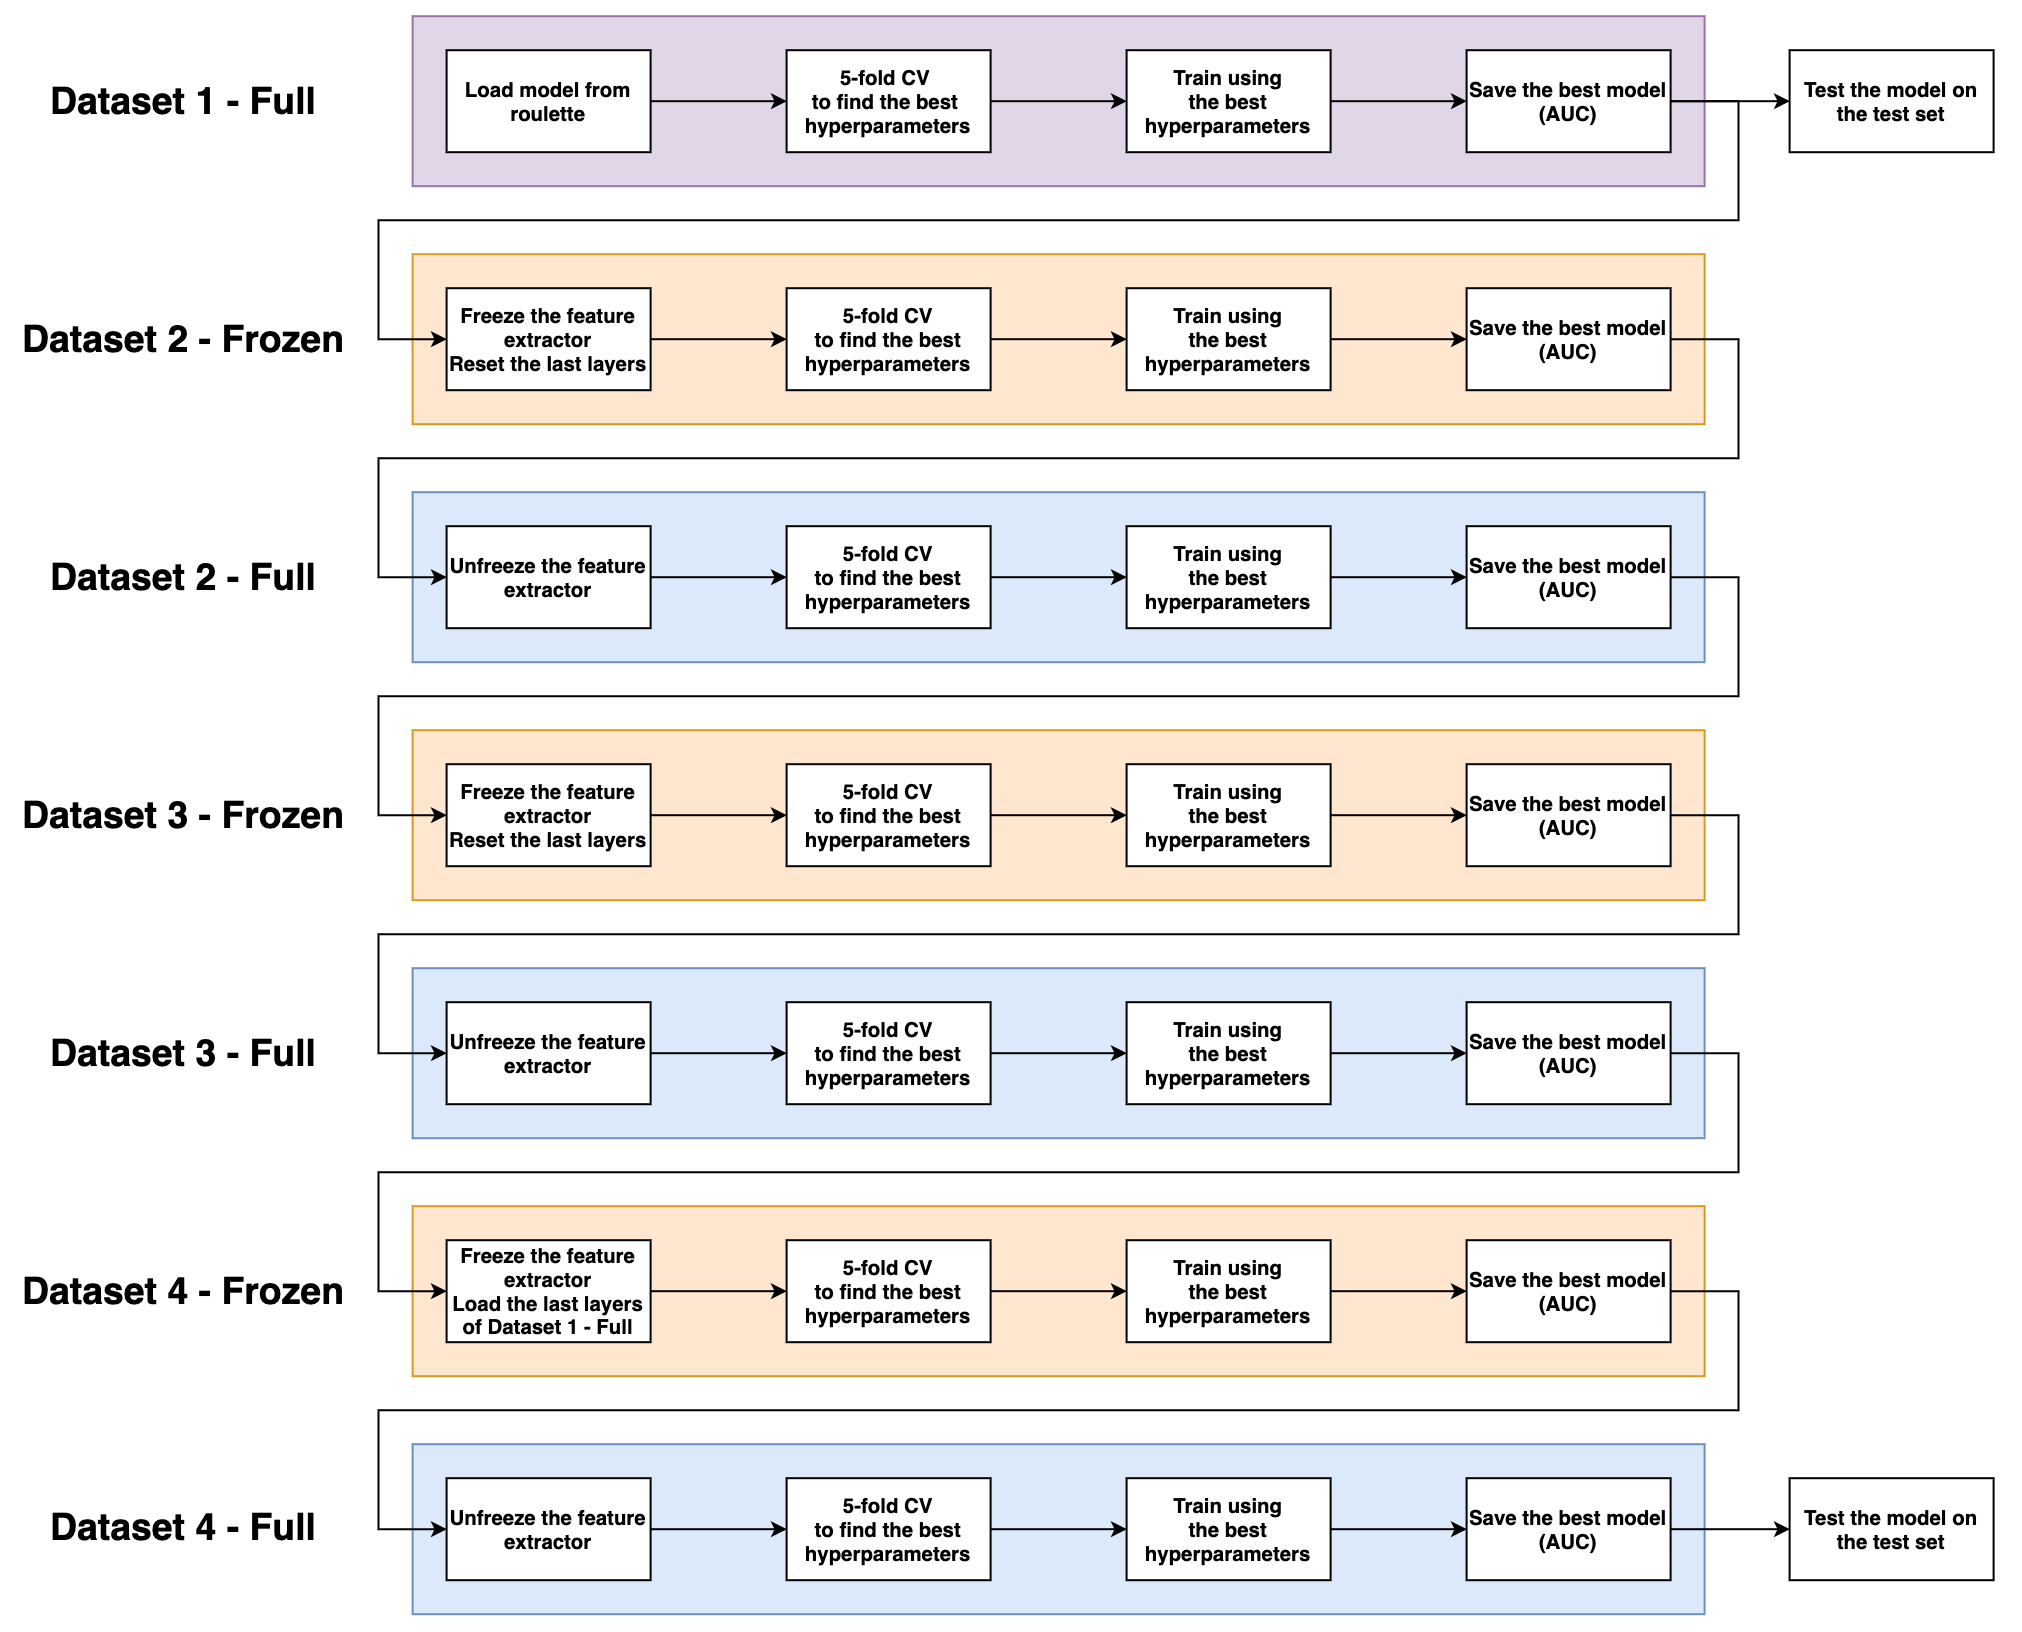
\includegraphics[width=1\textwidth, keepaspectratio=true]{./figures/tl_overview.png}
}
\caption{Transfer learning - Overview}
\label{fig:tl_overview}
\end{figure}


\section{Data processing}
\subsection{PROSTATEx}
\label{sec:PROSTATEx}
\setlength{\marginparwidth}{3cm}\leavevmode \marginnote{\textbf{Cl{\'e}ment}}Ideally, transfer learning should rely on multi-sequence MRIs only. In fact, the extra information provided by different sequences increases the performance a lot. However, publicly available datasets either do not contain the clinical significance of the samples or were purely made for segmentation purposes (where labels are also images).

As the other datasets used in this work do not contain multi-sequence exams (single-sequence MRIs and CT scans), it was required to extract single channel images from the PROSTATEx dataset. DWI images were selected because lesions are white on this sequence, as well as on CT scans. Hence, choosing DWI images ensured a consistent representation of tumors from one dataset to the other, which helps the cancer detection.

The overall process is the same as the one described in section \ref{sec:numpyToAugmentedStacked}, apart from a few details. First, a T2-weighted image was still used to align and resize the corresponding DWI image, but was not exported at the end, resulting in a single-channel DWI image (NumPy array) instead of stacked images. As DWI images are not of the same size, the fact of using the corresonding T2 images to resize them was the easiest way to make the new implementation go without a hitch.

Second, the way of cropping images was slighty modified. Previously, a 65x65px patch centered on the lesion was cropped, which sometimes resulted in patches cropped inside the lesion (i.e. patches which did not contain the entire lesion). As the two missing channels reduce the amount of information contained in each image, cropping inside lesions complicates the work of the neural network. Therefore, a larger patch of 130x130px was cropped, before being resized to 65x65px using a bicubic interpolation. These dimensions were found to be the best compromise across the whole dataset since they allowed to crop the vast majority of lesions with a small tissue margin around them. Consequently, the borders of the lesions are also visible on the images, which should help the detection process. 


\subsection{LungCTChallenge}
\label{sec:lungCTChallenge}
\subsubsection{Dataset description}
\setlength{\marginparwidth}{3cm}\leavevmode \marginnote{\textbf{Cl{\'e}ment}}Lung CT Challenge ~\cite{12, 36, 38} is composed of two different subdatasets of CT scans: one is called "calibration set" (10 patients) and the other "test set" (60 patients). Each patient can have one or multiple findings. Since labels were provided for both sets and the amount of data is fairly low, they were merged and used as a global training set. For each finding, an abnormal mass is visible in the lungs, which means that the classification is going to differentiate malignant from benign tumors.

Regarding labelling, two Excel files, \textit{TestSet\_NoduleData\_PublicRelease\_wTruth} and \textit{CalibrationSet\_NoduleData}, contain labels for these images. In order to facilitate the handling of information in the code, two CSV files were manually created: \mbox{\textit{TestSet.csv}} and \textit{CalibrationSet.csv}.
Contrary to PROSTATEx, more than two labels were used in this dataset. Both "malignant" and "Primary lung cancer" were considered as positive, whereas "benign" and "Benign nodule" were treated as negative. A third label called "Suspicious malignant nodule" appeared two times. Since the diagnosis was not clearly defined for those images, they were not included in the training data to avoid any noise. 


\subsubsection{From DICOM to augmented NumPy arrays}
\setlength{\marginparwidth}{3cm}\leavevmode \marginnote{\textbf{Cl{\'e}ment}}As PROSTATEx, the processing was split into two parts: preprocessing (DICOM to NumPy arrays) and augmentation (NumPy arrays to cropped augmented NumPy arrays.) Algorithm \ref{alg:LungCTChallenge_preprocessing} shows the various preprocessing steps.

The augmentation process is close to the one applied to PROSTATEx. An advantage Lung CT Challenge has is that all images have the same resolution (512x512 pixels), making the alignment process used for PROSTATEx useless. Nevertheless, lung tumors are particular. What differentiates them from the others is their look. In fact, lung tumors usually look like spider webs with a central nodule and branches coming out of it, whereas brain and prostate tumors tend to have well-defined boundaries. Therefore, a larger patch size was chosen in order to keep the extra information provided by the branches in the peripheral tissue. Furthermore, a perfect cropping method would only crop the interesting part of the tissue and a margin around it. However, tumor size varies a lot. It can either be extremely small (a dot) or large (massive nodule with long branches). Consequently, the selected patch size makes the largest tumors fit perfectly in the cropped area, inducing more tissue for smaller tumors. Naturally, there were few outliers whose size was a lot larger than the chosen patch size. If the patch size was set accordingly, entire lungs were sometimes visible in other patients' case. For this reason, these large tumors were treated as outliers. The chosen dimensions are 1/6 of the image width and height (i.e. 85x85px since the image size is 512x512px). These patches were then resized to 65x65px thanks to a bicubic interpolation, before being exported as NumPy arrays.

Also, and contrary to PROSTATEx, the dataset was more or less balanced (39 positives and 42 negatives). Therefore, each class was augmented the same amount of times (240x). Lastly, images were normalized with respect to Equation \ref{eq:normalization}. The mean and standard deviation were computed over the whole dataset. 

\begin{algorithm}
    \caption{Lung CT Challenge preprocessing}
    \label{alg:LungCTChallenge_preprocessing}
    \begin{algorithmic}[1] % The number tells where the line numbering should start
        \Procedure{main}{$dataset\_folder, train\_CSV, test\_CSV, output\_folder$}
        		\State Create output directories: $"output\_folder/True", "output\_folder/False"$\\
        		\State $csv\_training \gets read\_CSV(train\_CSV)$ \Comment{CalibrationSet.csv}
        		\State $csv\_test \gets read\_CSV(test\_CSV)$ \Comment{TestSet.csv}
            \State $csv\_concatenated \gets concat(csv\_training, csv\_test)$\Comment{Both CSV files contain similar information about different patients.}\\
            \For{$row$ in $csv\_concatenated$}
            		\State $patient\_id \gets row["Scan\ Number"]$
            		\State $slice\_number \gets row["Nodule\ Center\ Image"]$ \Comment{Value in $[1,\infty]$}
            		\State $finding\_id \gets row["Nodule\ Number"]$
            		\State $clinical\_significance \gets row["Diagnosis"]$\\
            		\If{$clinical\_significance$ == $"malignant"$ or $"Primary\ lung\ cancer"$}
            			\State{$clinical\_significance \gets True$}
            		\ElsIf{$clinical\_significance$ == $"benign"$ or $"Benign\ nodule"$}
            			\State{$clinical\_significance \gets False$}
            		\ElsIf {$clinical\_significance$ == $"Suspicious\ malignant\ nodule"$}
            			\State{Continue}
            		\EndIf\\
                \For{$visit\ in\ patient\_id$'s folder}
                		\For{$mri\_type$ in $visit$}
                			\For{$dicom\_file$ in $mri\_type$}
                				\If {$slice\_number == dicom\_file.InstanceNumber$}
                					\State{$slice \gets normalize\_dicom(dicom\_file)$} \Comment{see section \ref{sec:dicom_data_manipulation}}
                					\State{Save $slice$ in $"output\_folder/clinical\_significance"$}
                				\EndIf
                			\EndFor
            			\EndFor
            		\EndFor
            \EndFor
        \EndProcedure
    \end{algorithmic}
\end{algorithm}


\subsection{Kaggle Brain}
\label{sec:kaggleBrain}
\subsubsection{Dataset description}
\setlength{\marginparwidth}{3cm}\leavevmode \marginnote{\textbf{Cl{\'e}ment}}This dataset is publicly available on Kaggle~\cite{51}. All images come from single-sequence MRIs. It is composed of two folders: one containing images with cancerous tumors and another one containing images either without tumor or with a non-cancerous tumor. Images whose quality was extremely low (resolution, picture of a screen, artefacts, etc.) were manually removed. In other cases, the image quality was good but disturbing objects such as left/right markers, arrows pointing the tumor, etc. were visible. These objects were manually removed using the object removal tool in Photoshop or by cropping the image if the disturbing object was far from the skull. File names and file formats were heterogeneous. At the end of this process, the dataset was composed of 96 benign lesions and 133 malignant ones.


\subsubsection{Ground truth creation}
\label{sec:braingroundtruth}
\setlength{\marginparwidth}{3cm}\leavevmode \marginnote{\textbf{Cl{\'e}ment}}The particularity of this dataset is that no information apart from the clinical significance is provided. Therefore, it was necessary to create a ground truth CSV file from scratch so that the same processing methods as the other datasets could be applied to this one.

The first step was to standardize the file names and formats. The chosen convention is "$[yes|no]{index}.jpg$". The vast majority of the files were in the JPG file format, so the few PNG images were converted. Then, a CSV file containing the following columns was created: "PatientID", "Nodule Center Position", "fid", "Diagnosis". The "PatientID" is the filename without extension that was set during the first step (for example "$yes99$" or "$no3$"). The "Nodule Center Position" represents the pixel coordinates of the lesion. Fortunately, brain tumors are clearly visible on brain MRIs, which eased the process. To find the coordinates, every single image was opened at its original size in an image visualization software. A rectangle selection tool was used to draw a rectangle from the top left corner of the image (because the top left pixel corresponds to the pixel at the coordinates $(0,0)$ in NumPy arrays) to the center of the lesion. The pixel width and height of this rectangle gave the "i,j" coordinates of the lesion. These coordinates were reported manually. Then, the "fid" corresponds to the Finding ID. This parameter would be more pertinent if the same "PatientID" could have multiple findings, i.e. if the same patient could have multiple tumors. Since this information is made use of during the image processing of the other datasets, it was also added here. In this particular case, the "fid" was always set to "1". Finally, the "Diagnosis" was defined as "False" or "True" according to the folder which the image was in. This allows to simply use the same processing techniques as it is done for the other datasets.


\subsubsection{From JPG to NumPy arrays}
\setlength{\marginparwidth}{3cm}\leavevmode \marginnote{\textbf{Cl{\'e}ment}}Images had to be converted to single-channel NumPy arrays (grayscale) so that the values could be normalized further on. First, a mere conversion involving no content modification apart from going from three to one channel was performed. Second, images were normalized according to Equation \ref{eq:normalization}. The mean and standard deviation were computed over the whole dataset. Both classes were augmented by a common factor (200x) since both classes contain a relatively close number of instances (133 positives and 96 negatives).

Similarly to Lung CT Challenge, tumor sizes vary substantially. The same methodology was applied regarding the patch size, i.e. choosing a size which fits the majority of large tumors perfectly. Even though the images all show the head under the same perspective (same height/width ratio, visible skull, black margin around the skull), images were probably collected from different sources, which explains the heterogeneity of resolutions. As a consequence, the patch size could not be a fixed number of pixels for all images because the cropped area would be the entire head on one image and a small portion of the tumor on another. The trick consisted in finding the horizontal and vertical portions of the image occupied by the tumor. In fact, cropping an area centered on the lesion whose height was $\frac{2}{7}$ of the image and whose width was $\frac{1}{4}$ gave good results. Finally, images were also resized to 65x65px using a bicubic interpolation before being saved as NumPy arrays. 


\subsection{Image cropping}
\setlength{\marginparwidth}{3cm}\leavevmode \marginnote{\textbf{Cl{\'e}ment}}Multiple ways of cropping images were tested out. The differences lay in how much tissue was kept around the lesion. In some cases, more context around the lesion allows to capture details about the connections between the lesion and blood vessels for example. Moreover, the abrupt borders inducing a clear change of colors can help detect tumors. Experienced showed that more context helps when the images are single-sequence. On the other hand, cropping right around the lesion or even in the lesion gave better results for multi-sequence data, i.e. when T2-weighted, DWI and ADC images (MRIs) were simultaneously used to perform the tumor detection and classification. In the latter case, the lesion usually appears distinctively on the three sequences, and this impacts the decision a lot. On single-sequence images, there is a clear lack of information which makes it difficult to differentiate a tumor from another tissue without much context. 


\subsection{Verification}
\subsubsection{Visual checking}
\setlength{\marginparwidth}{3cm}\leavevmode \marginnote{\textbf{Cl{\'e}ment}}Regarding the Kaggle brain dataset, the data generated was paid close attention to since the ground truth CSV file was created by hand (see Section \ref{sec:braingroundtruth}). In fact, each generated image was taken a close look at, which allowed to spot 3 mistakes over the whole dataset. They concerned typos in the "Nodule Center Position", which created pitch black images since the cropped area was outside.
Like PROSTATEx (see section \ref{sec:dataProcessingVerification}), control images with red dots were also generated for the other datasets. 


\section{Transfer learning implementation}
\subsection{Architecture generalities}
\subsubsection{Layer freezing}
\setlength{\marginparwidth}{3cm}\leavevmode \marginnote{\textbf{Cl{\'e}ment}}After each dataset switch, the model is first trained with freezed layers. The freezed layers are those considered as feature extractor, i.e. the first layers of the model. The exact point where the model is split is arbitrary, but is usually located after the convolutions. To perform this freezing, multiple steps are required:
\begin{enumerate}
	\item Reset the last layers. To do so, an instance of the model is created by loading the state dictionary of the previous one, before replacing the module containing the last layers with a new instance. 
	\item Iterate over the batch normalization layers and freeze them. Step 3 is not sufficient to freeze batch normalization layers. This can be achieved by calling module.eval() on each module containing such layers (after the model.train() call). 
	\item Only pass the parameters of these last layers to the optimizer.
\end{enumerate}

\noindent Figure \ref{fig:tl_model_split} shows the chosen model split for this experience. The first fully connected layer is part of the feature extractor because it can be considered as a feature gatherer and assembler. The next ones are part of the decision maker. 

\begin{figure}[!h]
\centering
\noindent
\makebox[\textwidth]{
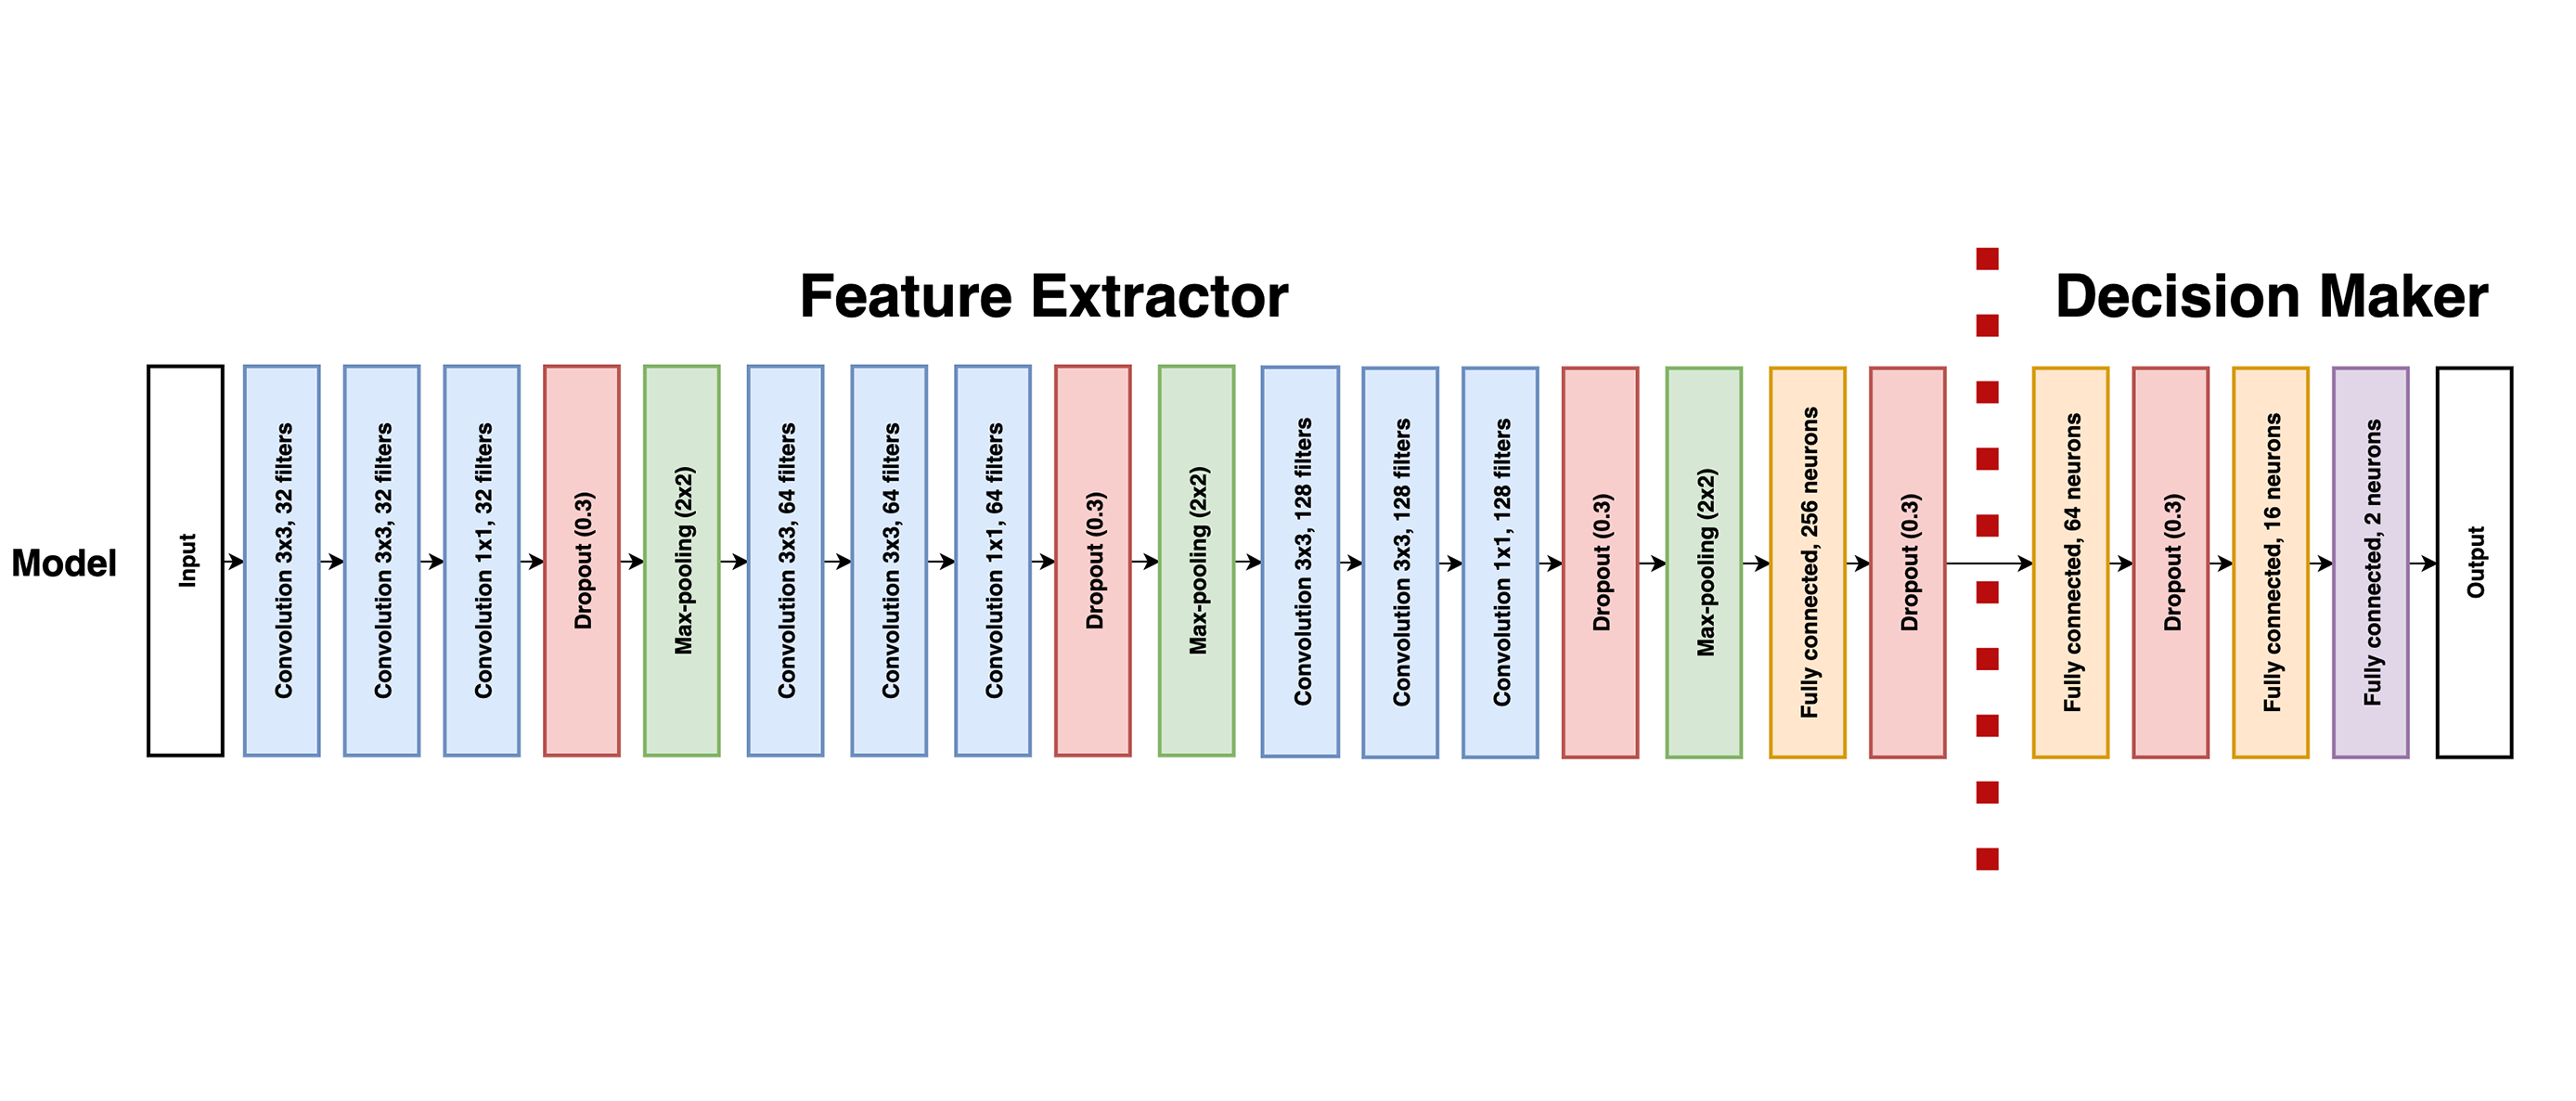
\includegraphics[width=1\textwidth, keepaspectratio=true]{./figures/tl_model_split.png}
}
\caption{Transfer learning - Model split}
\label{fig:tl_model_split}
\end{figure}


%\subsubsection{Parallelization}
%Each experiment before transfer learning was performed on a single GPU. While being a lot faster than training on a CPU, the computation time was still relatively high. In order to get results from the transfer learning in a reasonable amount of time, parallelization was required. In fact, the longest transfer learning experiment consisted of $(5$ folds $* 4$ learning rates $* 1200$ epochs $+ 1200$ epochs$) * 7$ parts $= 176400$ epochs. On a single GPU, this experiment would have taken around two weeks to complete. 
%
%Thanks to parallelization, the cross-validation combinations could be run simultaneously on different GPUs (5 of them since 5-fold cross-validation was used). To achieve this while using Python and GPUs, we relied on a library called Ray. The function responsible for training the model needs to be defined as a Ray remote function thanks to a decorator (@$ray.remote$ above the function declaration). This new function does not return the actual return values, but object IDs pointing to placeholders for the future results, which allows to continue the execution and run other parallel functions. Outside of the cross-validation loop, a call to $ray.get()$ on the object IDs allows to wait for the simultaneous executions to complete and to collect the different results. 
%
%\begin{figure}[!h]
%\centering
%\noindent
%\makebox[\textwidth]{
%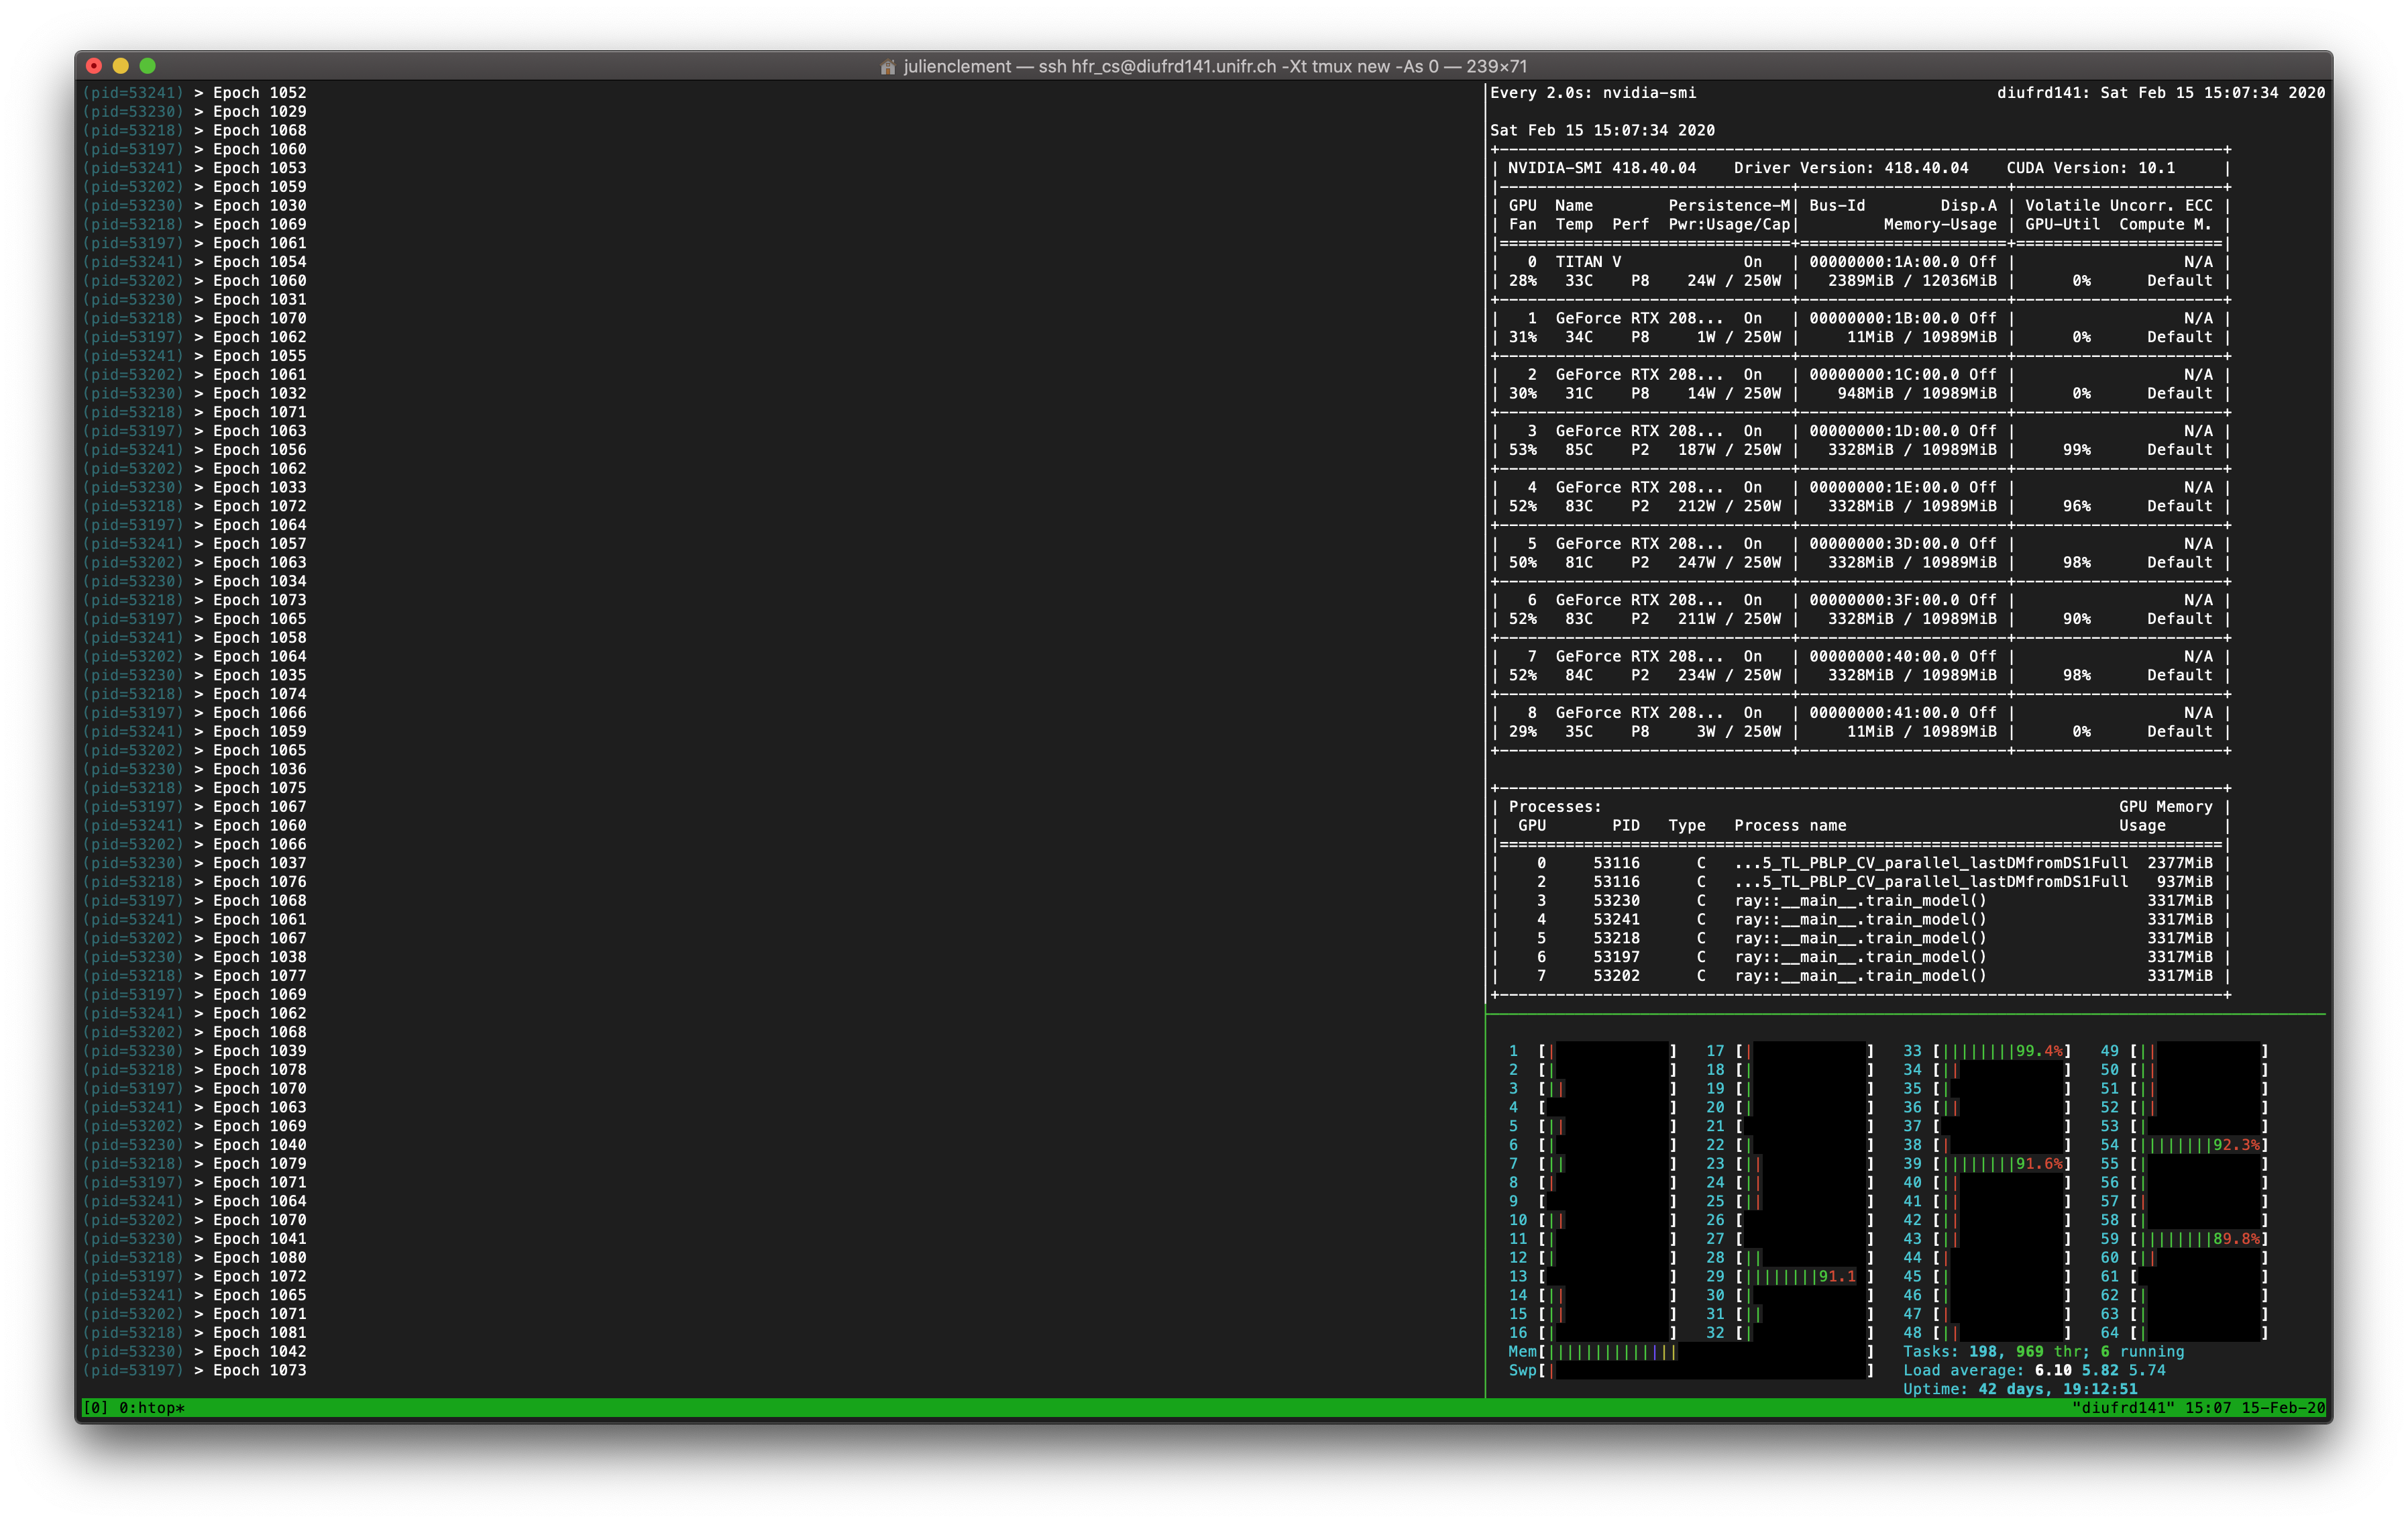
\includegraphics[width=1.3\textwidth, keepaspectratio=true]{./figures/tl_parallel_run.png}
%}
%\caption{Transfer learning - Parallelization}
%\label{fig:tl_parallel_run}
%\end{figure}


\subsection{Script options}
\setlength{\marginparwidth}{3cm}\leavevmode \marginnote{\textbf{Cl{\'e}ment}}A single Python script allows to run the entire transfer learning pipeline. Multiple command line arguments are required in order to load the right datasets and the right model, to define the hyperparameters, etc. Table \ref{fig:transfer_learning_options} gives a exhaustive list of the script options. The particularity lies in the learning rate, number of epochs, batch size and dropout options. In fact, the pipeline consists in seven different phases of training: dataset 1 (full model), dataset 2 (frozen model), dataset 2 (full), dataset 3 (frozen), dataset 3 (full), dataset 4 (frozen) and dataset 4 (full). In such a case, each phase will probably use different hyperparameters. Therefore, these command line options need to specify seven different parameters. For example, a valid value for the "--lr" option could be "1e-8,1e-5,1e-6,1e-6,1e-5,1e-7,1e-8".


% Please add the following required packages to your document preamble:
% \usepackage{graphicx}
% \usepackage[table,xcdraw]{xcolor}
% If you use beamer only pass "xcolor=table" option, i.e. \documentclass[xcolor=table]{beamer}
\begin{table}[!h]
\resizebox{\textwidth}{!}{%
\begin{tabular}{|llll|}
\hline
\rowcolor[HTML]{DAE8FC} 
\textbf{Command}            & \textbf{Description}                                                                                                                                                                                                & \textbf{Required}                                                           & \textbf{Type} \\ \hline
\textbf{--training-set1}     & Path to training set 1                                                                                                                                                                                                  & True                                                                        & String        \\ \hline
\textbf{--validation-set1}   & Path to validation set 1                                                                                                                                                                                                                                                                                                                                                                                                  & True                                                                        & String        \\ \hline
\textbf{--test-set1}     & Path to test set 1                                                                                                                                                                                                                                                                                                                                                                                                   & True                                                                        & String        \\ \hline
\textbf{--training-set2}     & Path to training set 2                                                                                                                                                                                                 & True                                                                        & String        \\ \hline
\textbf{--validation-set2}   & Path to validation set 2 
& True                                                                        & String        \\ \hline
\textbf{--training-set3}     & Path to training set 3                                                                                                                                                                                                  & True                                                                        & String        \\ \hline
\textbf{--validation-set3}   & Path to validation set 3                                                                                                                                                                                                                                                                                                                                                                                                  & True                                                                        & String        \\ \hline
\textbf{--batchsize}        & Number of samples per batch                                                                                                                                                                                         & True                                                                        & Comma-separated ints          \\ \hline
\textbf{--nbepochs}         & Number of epochs the training phase lasts                                                                                                                                                                  & True                                                                        & Comma-separated ints            \\ \hline
\textbf{--lr}               & Learning rate used in the optimizer                                                                                                                                                                                 & \begin{tabular}[c]{@{}l@{}}True\end{tabular}               & Comma-separated floats         \\ \hline
\textbf{--lossfunction}     & \begin{tabular}[c]{@{}l@{}}Loss function name\\{[}CrossEntropyLoss, L1Loss, MSELoss{]}\end{tabular}                                                                                                            & \begin{tabular}[c]{@{}l@{}}False\\ Default: 'CrossEntropyLoss'\end{tabular} & String        \\ \hline
\textbf{--cuda-device}      & GPU name to run the experiment                                                                                                                                                                                      & \begin{tabular}[c]{@{}l@{}}False\\ Default: 'cuda'\end{tabular}             & String        \\ \hline
\textbf{--modeltoload}      & \begin{tabular}[c]{@{}l@{}}Pretrained model name \\If given, load it, otherwise randomly initialize it\end{tabular}                                                                                     & \begin{tabular}[c]{@{}l@{}}False\\ Default: ""\end{tabular}                 & String        \\ \hline
\textbf{--dropout}          & Dropout probability                                                                                                                                                                                                 & \begin{tabular}[c]{@{}l@{}}True\end{tabular}                & Comma-separated floats          \\ \hline
\textbf{--optimized-metric} & \begin{tabular}[c]{@{}l@{}}Metric to optimize\\ The best model during the training will be saved according to it\\{[}'auc', 'accuracy', 'precision', 'recall', 'f1score', 'specificity'{]}\end{tabular} & \begin{tabular}[c]{@{}l@{}}False\\ Default: 'auc'\end{tabular}              & String        \\ \hline
\textbf{--outputdirectory}  & Root of the output directory used by Tensorboard to save the models                                                                                                                                                 & True                                                                        & String        \\ \hline
\textbf{--cv} & \begin{tabular}[c]{@{}l@{}}Whether to use cross-validation or not\\{[}'True', 'False'{]}\end{tabular} & \begin{tabular}[c]{@{}l@{}}True\end{tabular}             
& String        \\ \hline
\end{tabular}%
}
\caption{Complete list of script options}
\label{fig:transfer_learning_options}
\end{table}


\subsection{Visualization of the impact of the various datasets on the target task}
\label{sec:global_performance}
\setlength{\marginparwidth}{3cm}\leavevmode \marginnote{\textbf{Cl{\'e}ment}}The so-called global performance graphs are a visual representation of the impact of each part of the transfer learning and each dataset on the target task. On paper, each step of the transfer learning is supposed to make the model learn new features that are useful for the first dataset (the target dataset). As described in section \ref{sec:process_overview}, the model can be seen as a feature extractor and a decision maker. Hence, to see how much each step was actually helping the process, the decision maker resulting from the best model of the first step of the transfer learning, i.e. the training on the first/target dataset, was saved. As this decision maker is saved after the training on the target dataset, it is specialized in the classification of the latter. In other words, if the target dataset is a prostate dataset, it will classify prostate tumors with a relatively high precision.

Then, after each epoch of every other transfer learning step, the saved decision maker was attached to the current feature extractor. This temporary model was then tested on the target training and validation sets, which resulted in different training and validation metrics.

At the end of the transfer learning pipeline, a graph was generated for each metric. These curves show the evolution of the latter across the entire process, which allows to determine the impact of each non-target dataset on the target task. If a metric is increasing, the features learned thanks to the corresponding dataset are useful for the target one. In this case, the graphs show how much the features learned from each dataset help classify prostate lesions. 

%\subsection{Visualization of the impact of the various datasets on the target task}
%\label{sec:global_performance}
%\setlength{\marginparwidth}{3cm}\leavevmode \marginnote{\textbf{Julien}}On paper, each step of the transfer learning is supposed to make the model learn new features that are useful for the first dataset (the target dataset). As described in section \ref{sec:process_overview}, the model can be seen as a feature extractor and a decision maker. Hence, to see how much each step was actually helping the process, the decision maker resulting from the first step of the transfer learning, i.e. the training on the first/target dataset, was saved. As this decision maker is saved after the training on the target dataset, it is specialized in the classification of the latter. In other words, if the target dataset is a prostate dataset, it will classify prostate tumors with a relatively high precision. 
%
%Then, after each epoch of every other transfer learning step, the saved decision maker was attached to the current feature extractor. This temporary model was then tested on the target training and validation sets, which resulted in different training and validation metrics. 
%
%At the end of the transfer learning pipeline, a graph was generated for each metric. These curves show the evolution of the latter across the entire process, which allows to determine the impact of each non-target dataset on the target task. If a metric is increasing, the features learned thanks to the corresponding dataset are useful for the target one. Figure \ref{fig:global_performance_example} shows an example of this graph for the AUC.\\
%As expected, the curve is flat during the frozen parts. Since the same decision maker is attached to frozen layers (which remain the same by definition), the values of the metrics do not change at all. 
%
%\begin{figure}[!h]
%\centering
%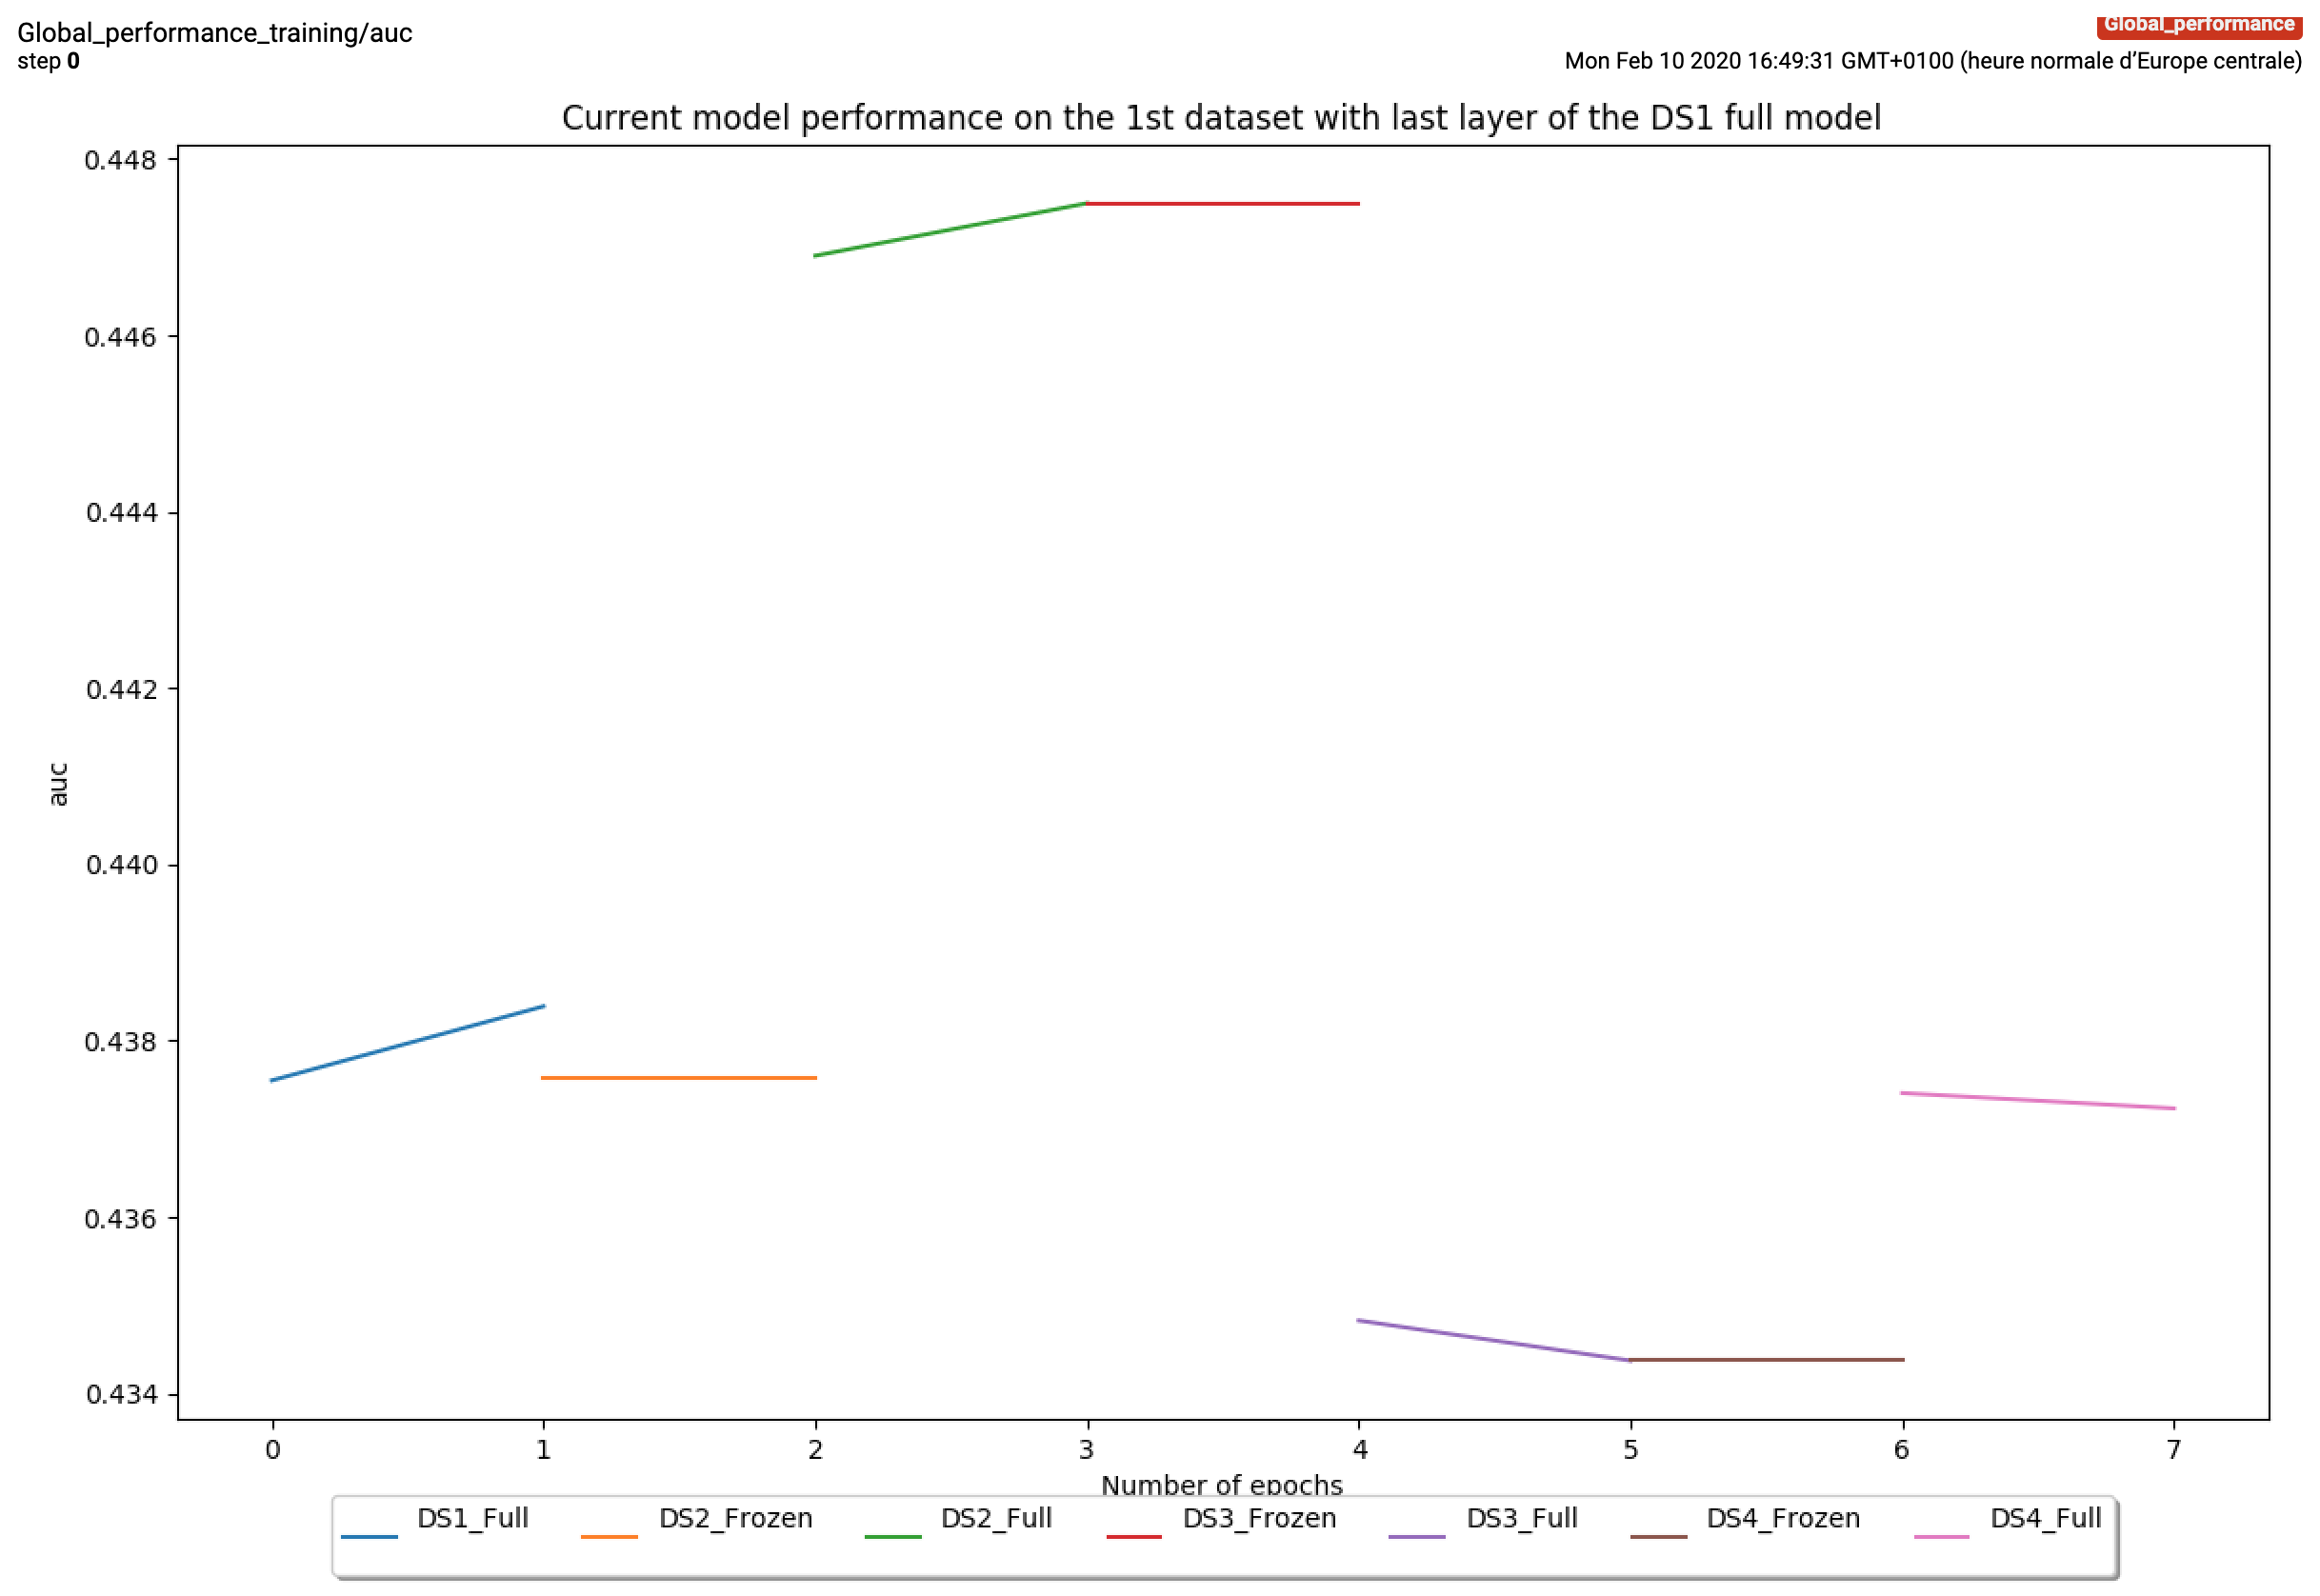
\includegraphics[width=1\textwidth, keepaspectratio=true]{./figures/global_performance_example.png}
%\caption{Please replace this figure with a real example as soon as the results are available!}
%\label{fig:global_performance_example}
%\end{figure}


\subsection{Experimental setup}
\setlength{\marginparwidth}{3cm}\leavevmode \marginnote{\textbf{Jobin}}The whole transfer learning consists in multiple steps. In order to maximize the performance during the whole process, the hyperparameters were manually tuned at each step, following a grid search approach to find the best ones. Table \ref{table:tl_hyperparameters_at_each_step} presents the best hyperparameters used at each step of the experiment. Note that, as it was the case in the paper experiment reproduction, the first model was also initialized by loading the best model among 200 initializations. The model was implemented with PyTorch using the Adam optimizer to update its weights. The complete succession of the process took approximately 60 hours on an Nvidia GeForce RTX 2080 Ti. 
%Tesla v100 XSM2 graphics card.

\begin{table}[!h]
\resizebox{\textwidth}{!}{%
\begin{tabular}{|l|l|c|l|c|l|}
\hline
\rowcolor[HTML]{DAE8FC} 
\textbf{Dataset}         & \multicolumn{1}{c|}{\cellcolor[HTML]{DAE8FC}\textbf{Step}} & \textbf{Learning rate} & \multicolumn{1}{c|}{\cellcolor[HTML]{DAE8FC}\textbf{Batch size}} & \textbf{Dropout} & \textbf{Number of epochs} \\ \hline
\textbf{PROSTATEx}       & DS1/Full                                                   & 1e-8                   & 128                                                              & 0.4              & 2000                      \\ \hline
\textbf{Kaggle Brain}    & DS2/Frozen                                                 & 1e-7                   & 128                                                              & 0.3              & 2000                      \\ \hline
\textbf{Kaggle Brain}    & DS2/Full                                                   & 1e-8                   & 128                                                              & 0.3              & 2000                      \\ \hline
\textbf{Lung CT Challenge} & DS3/Frozen                                                 & 1e-5                   & 128                                                              & 0.3              & 2000                      \\ \hline
\textbf{Lung CT Challenge} & DS3/Full                                                   & 1e-8                   & 128                                                              & 0.3              & 2000                      \\ \hline
\textbf{PROSTATEx}       & DS4/Frozen                                                 & 1e-5                   & 128                                                              & 0.3              & 2000                      \\ \hline
\textbf{PROSTATEx}       & DS4/Full                                                   & 1e-9                   & 128                                                              & 0                & 2000                      \\ \hline
\end{tabular}%
}
\caption{Hyperparameters used at each step of the transfer learning pipeline}
\label{table:tl_hyperparameters_at_each_step}
\end{table}


\section{Results}

%\subsection{Independent training}
%To get reference values and evaluate the impact of transfer learning on the model performance, a set of trainings on each dataset was performed independently. These experiments involved multiple hyperparameter combinations. The best results were used as benchmark values. 
%
%\subsubsection{PROSTATEx}
%
%\subsubsection{Kaggle brain}
%
%\subsubsection{Lung CT Challenge}


%\subsection{Transfer learning}
\setlength{\marginparwidth}{3cm}\leavevmode \marginnote{\textbf{Jobin \& Cl{\'e}ment}}Figures \ref{fig:tl_ds1_full} to \ref{fig:tl_ds4_full} show the performance of the model at each step of the transfer learning. Each graph displays the metric values achieved on the training and the validation set on the Y-axis, whereas the X-axis represents the number of epochs.
Table \ref{table:tl_best_model_performance} summaries the performance of the best model on the validation and test sets at each step of the experiment. 
Finally, Figure \ref{fig:tl_results_test_set} compares the performance of the model resulting from the first training to the one which underwent the transfer learning experiment. 

\newpage 

\begin{figure}[!h]
\centering
\noindent
\makebox[\textwidth]{
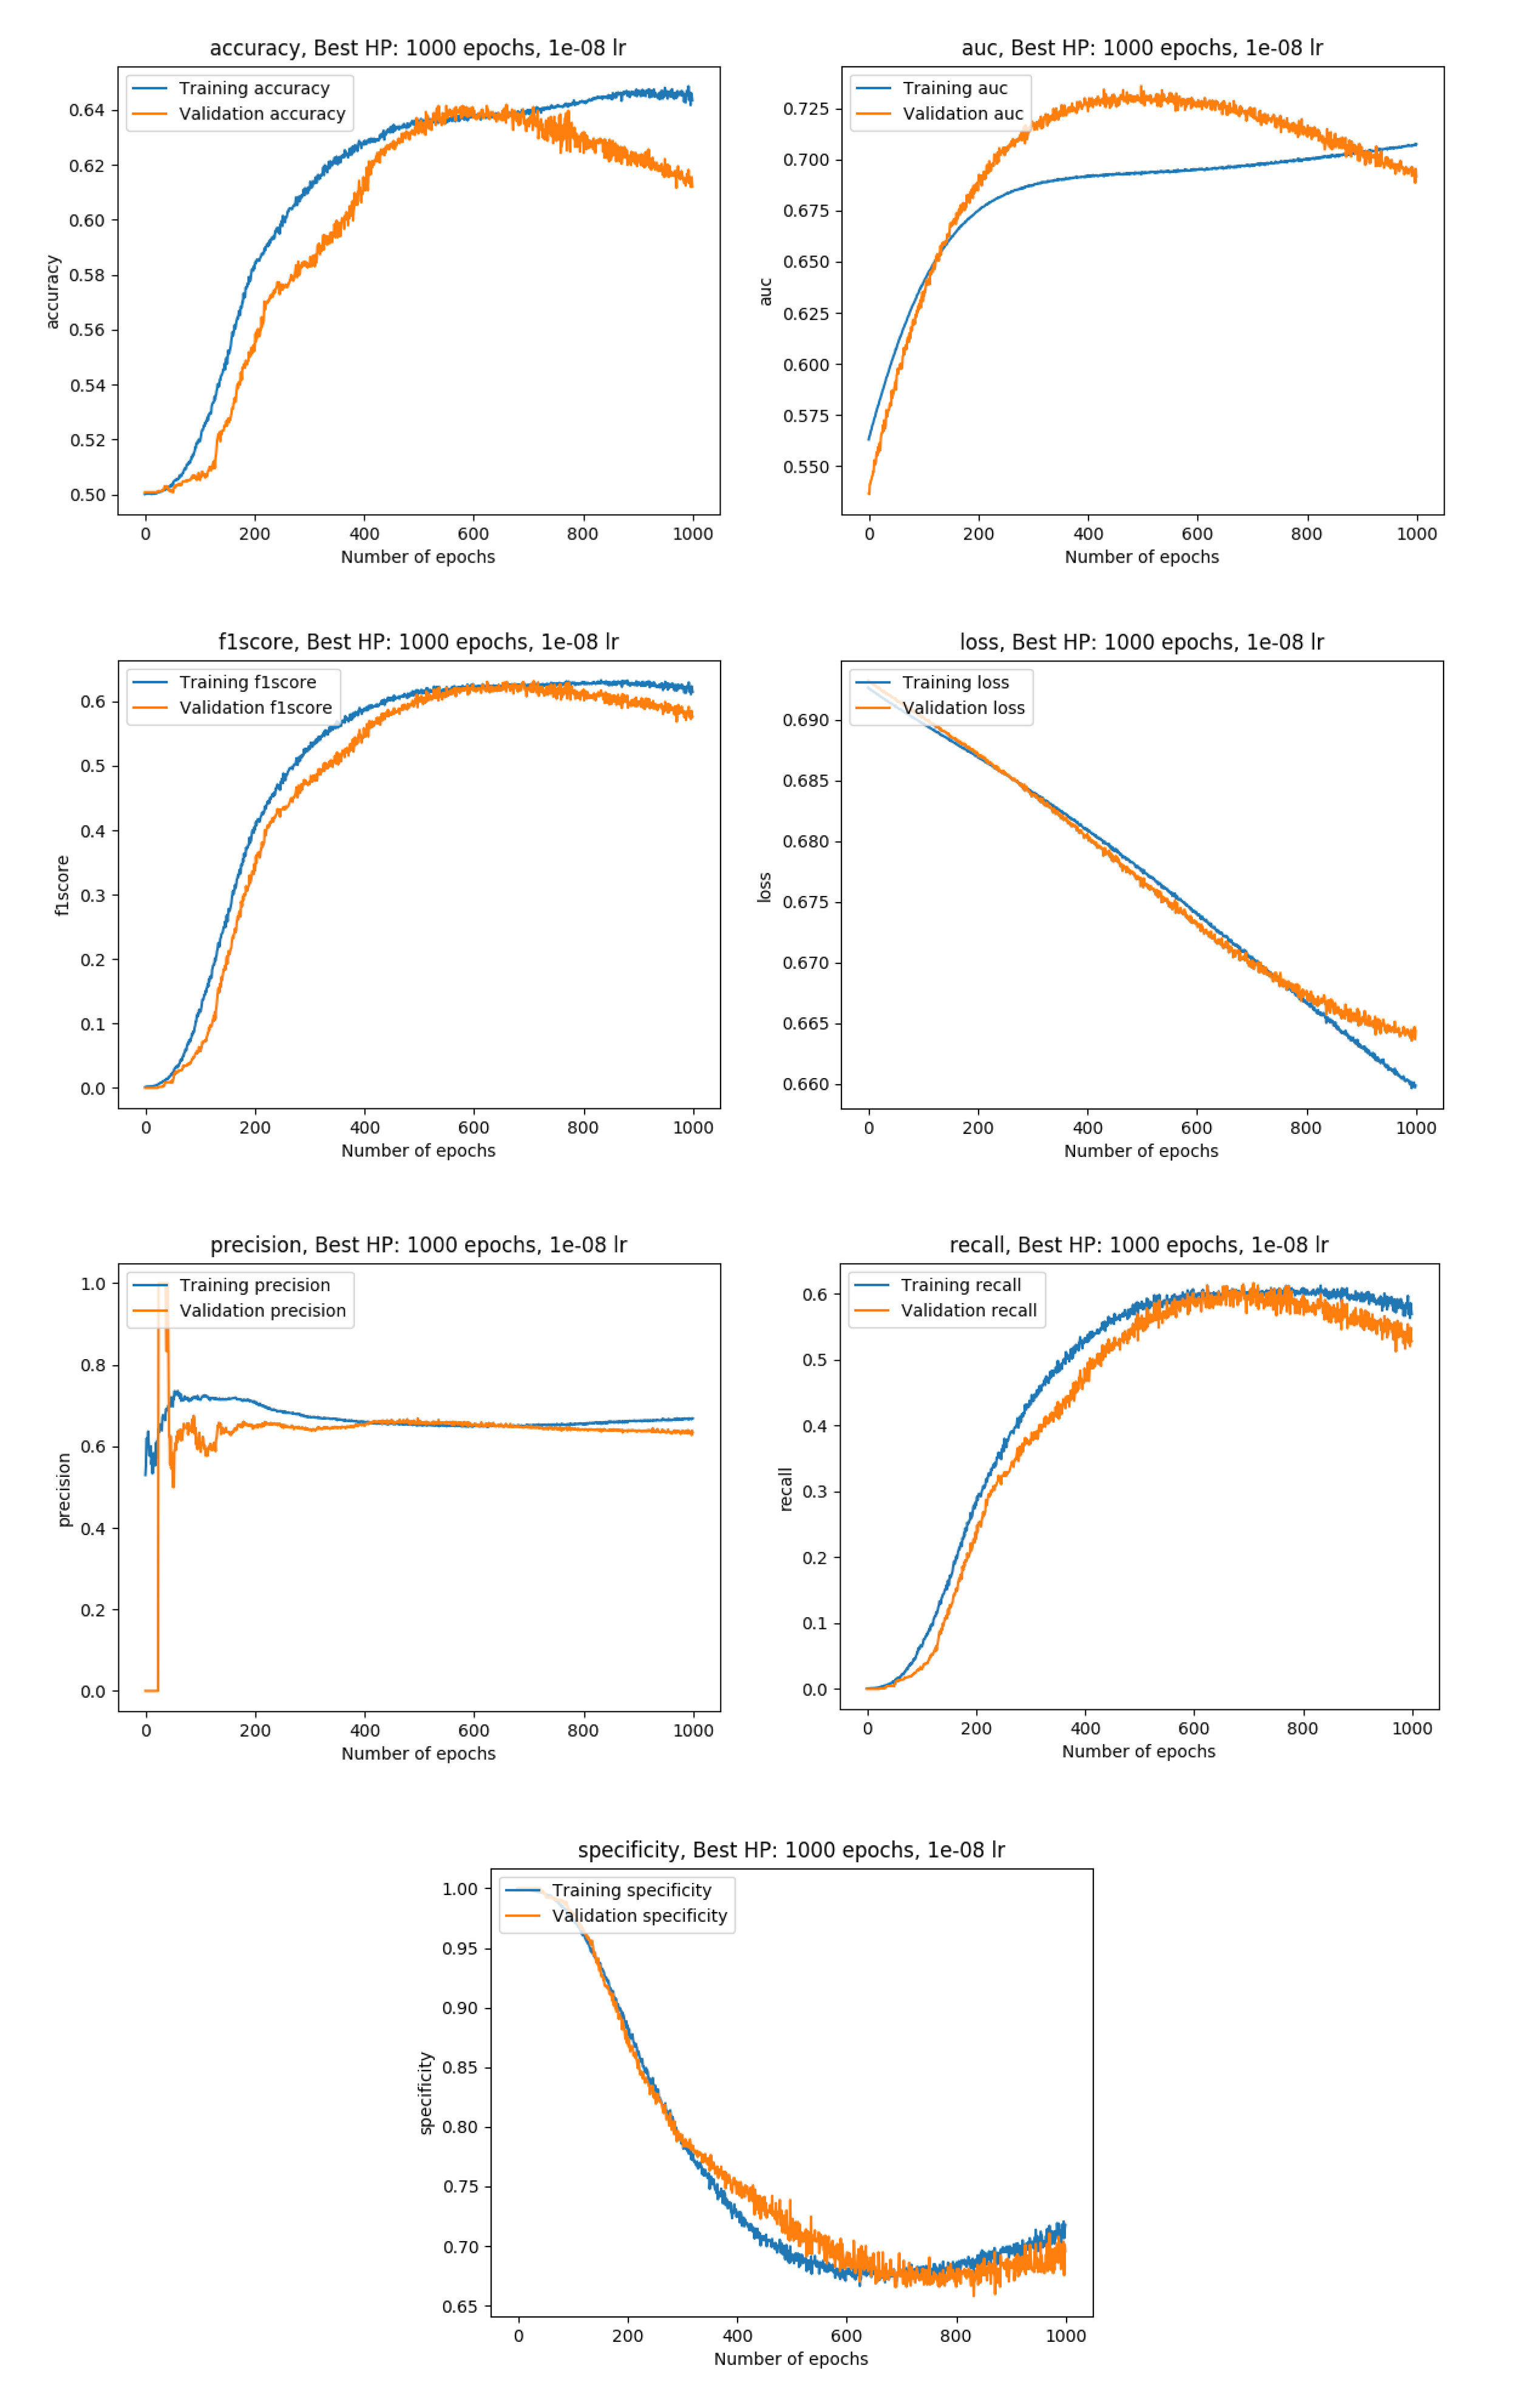
\includegraphics[width=1\textwidth, keepaspectratio=true]{./figures/tl_DS1_full.png}
}
\caption{Transfer learning - DS1 Full}
\label{fig:tl_ds1_full}
\end{figure}

\begin{figure}[!t]
\centering
\noindent
\makebox[\textwidth]{
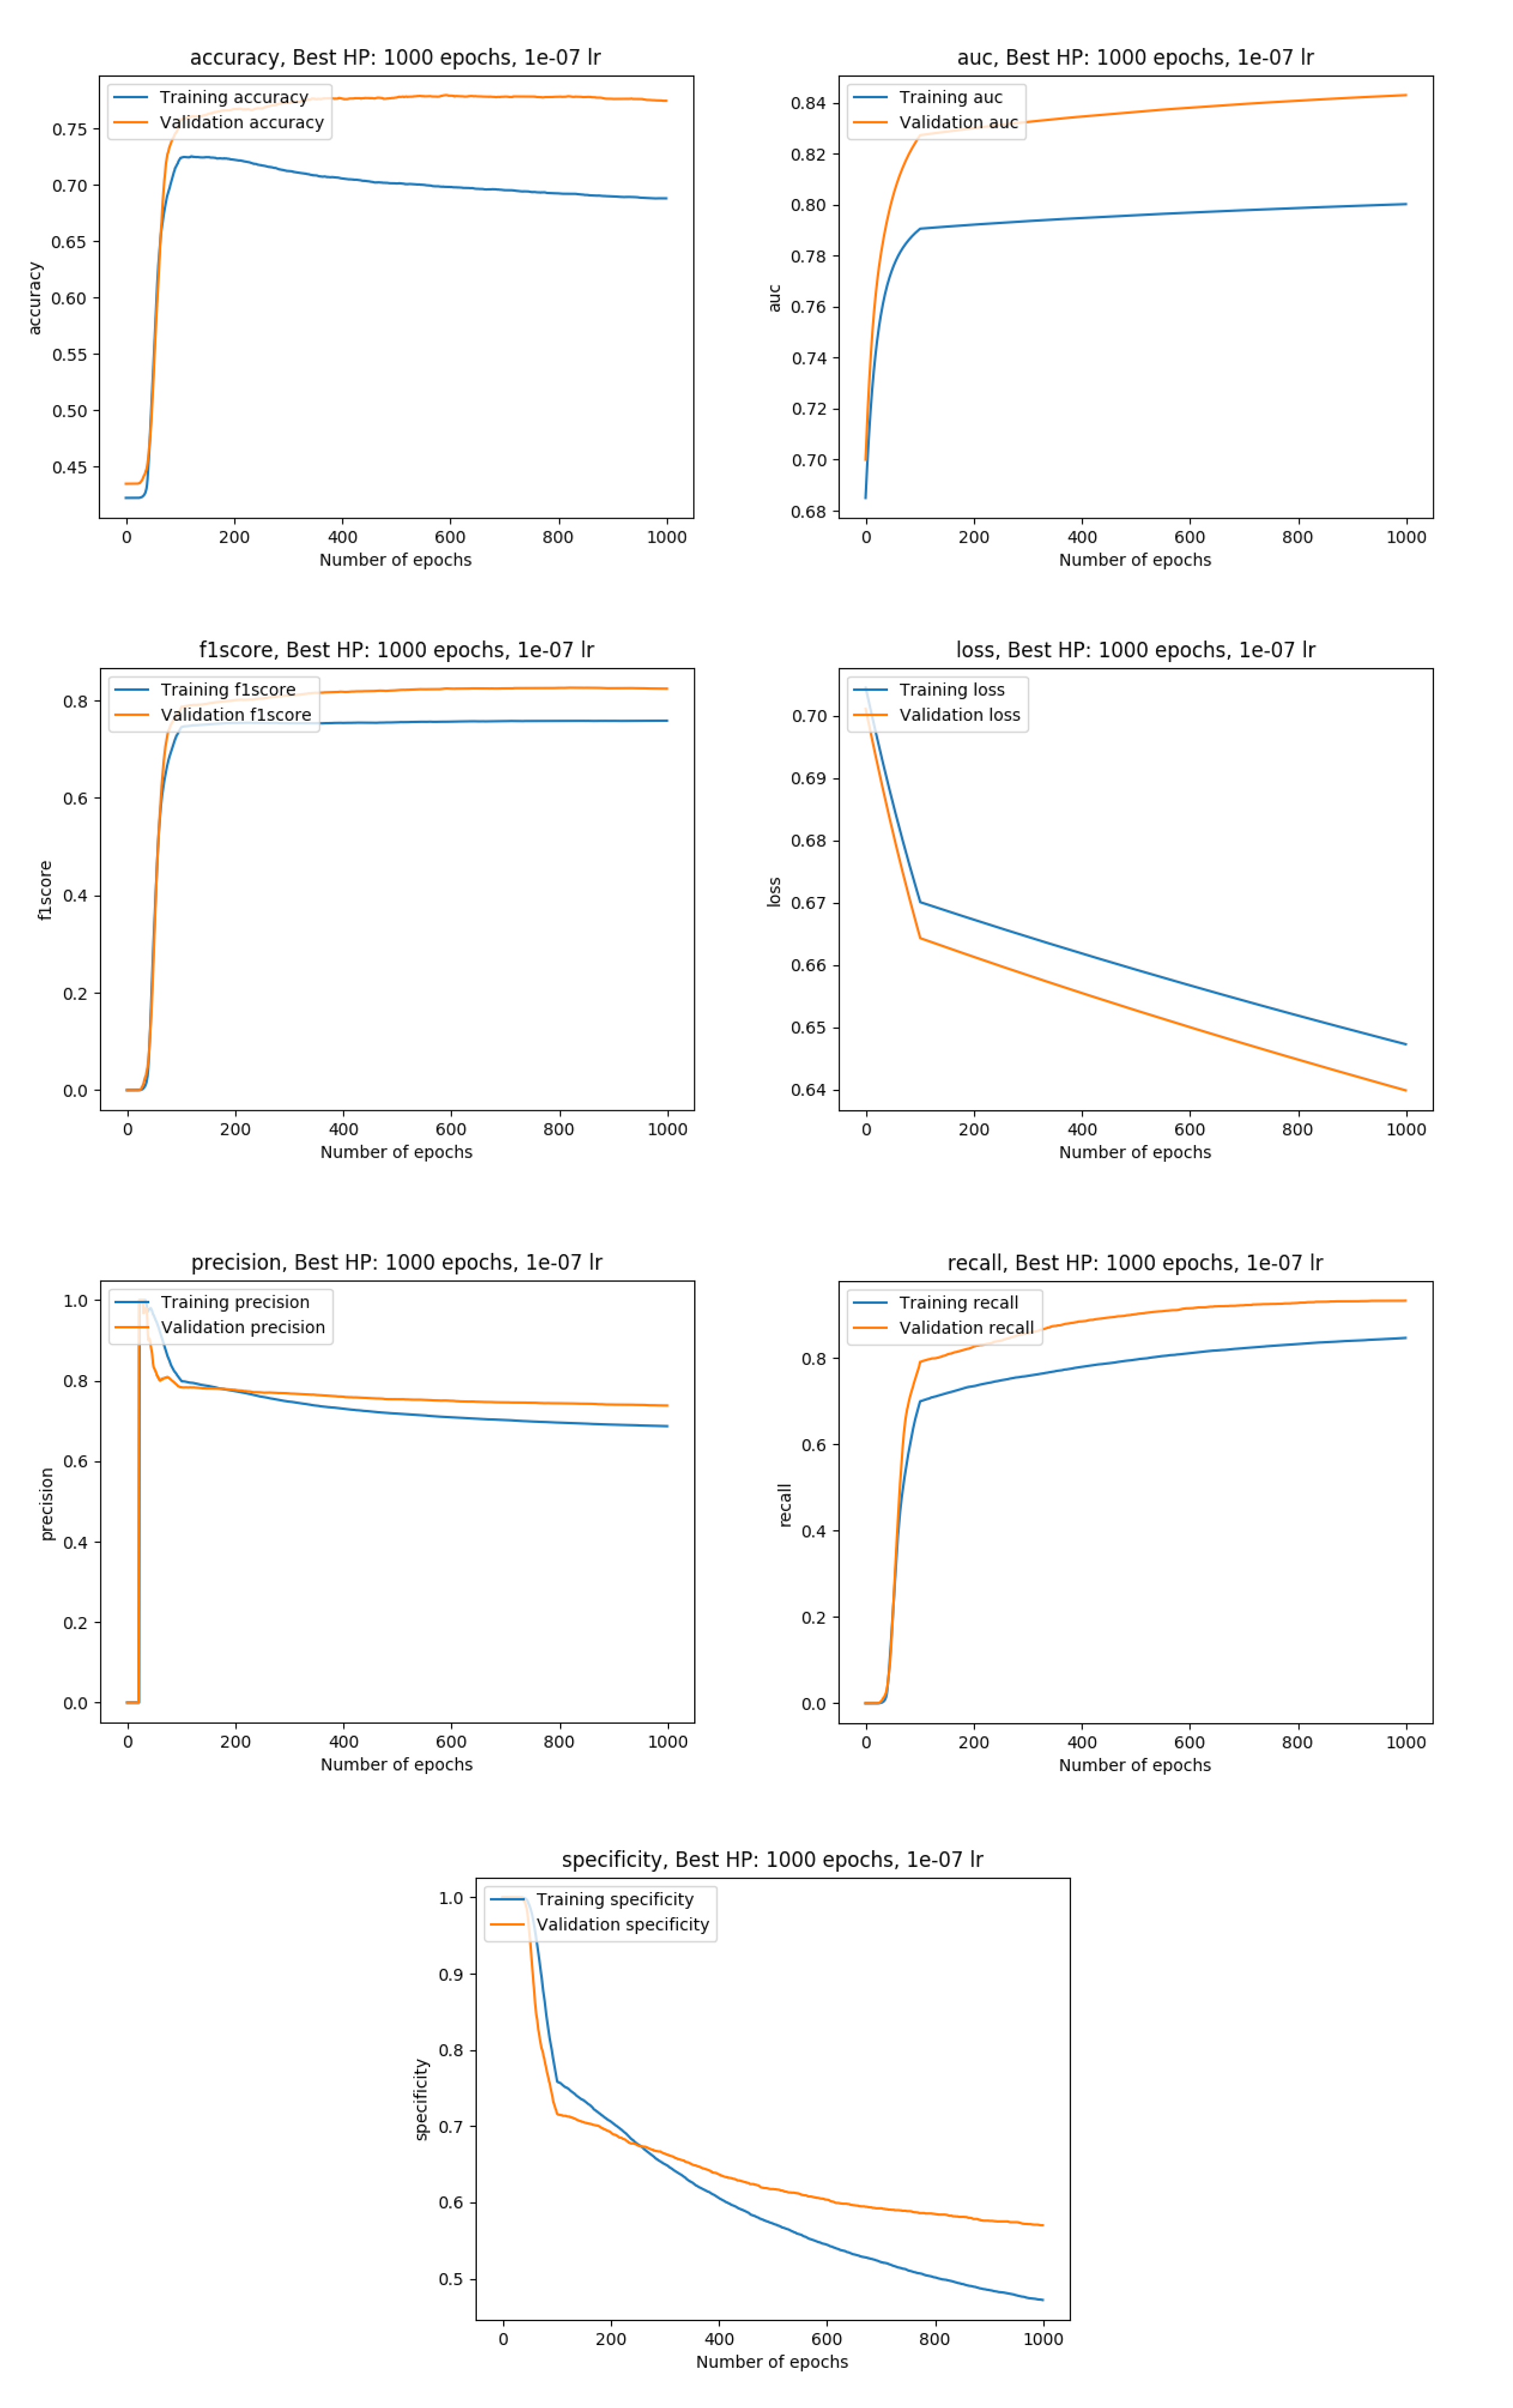
\includegraphics[width=1\textwidth, keepaspectratio=true]{./figures/tl_DS2_frozen.png}
}
\caption{Transfer learning - DS2 Frozen}
\label{fig:tl_ds2_frozen}
\end{figure}

\begin{figure}[!t]
\centering
\noindent
\makebox[\textwidth]{
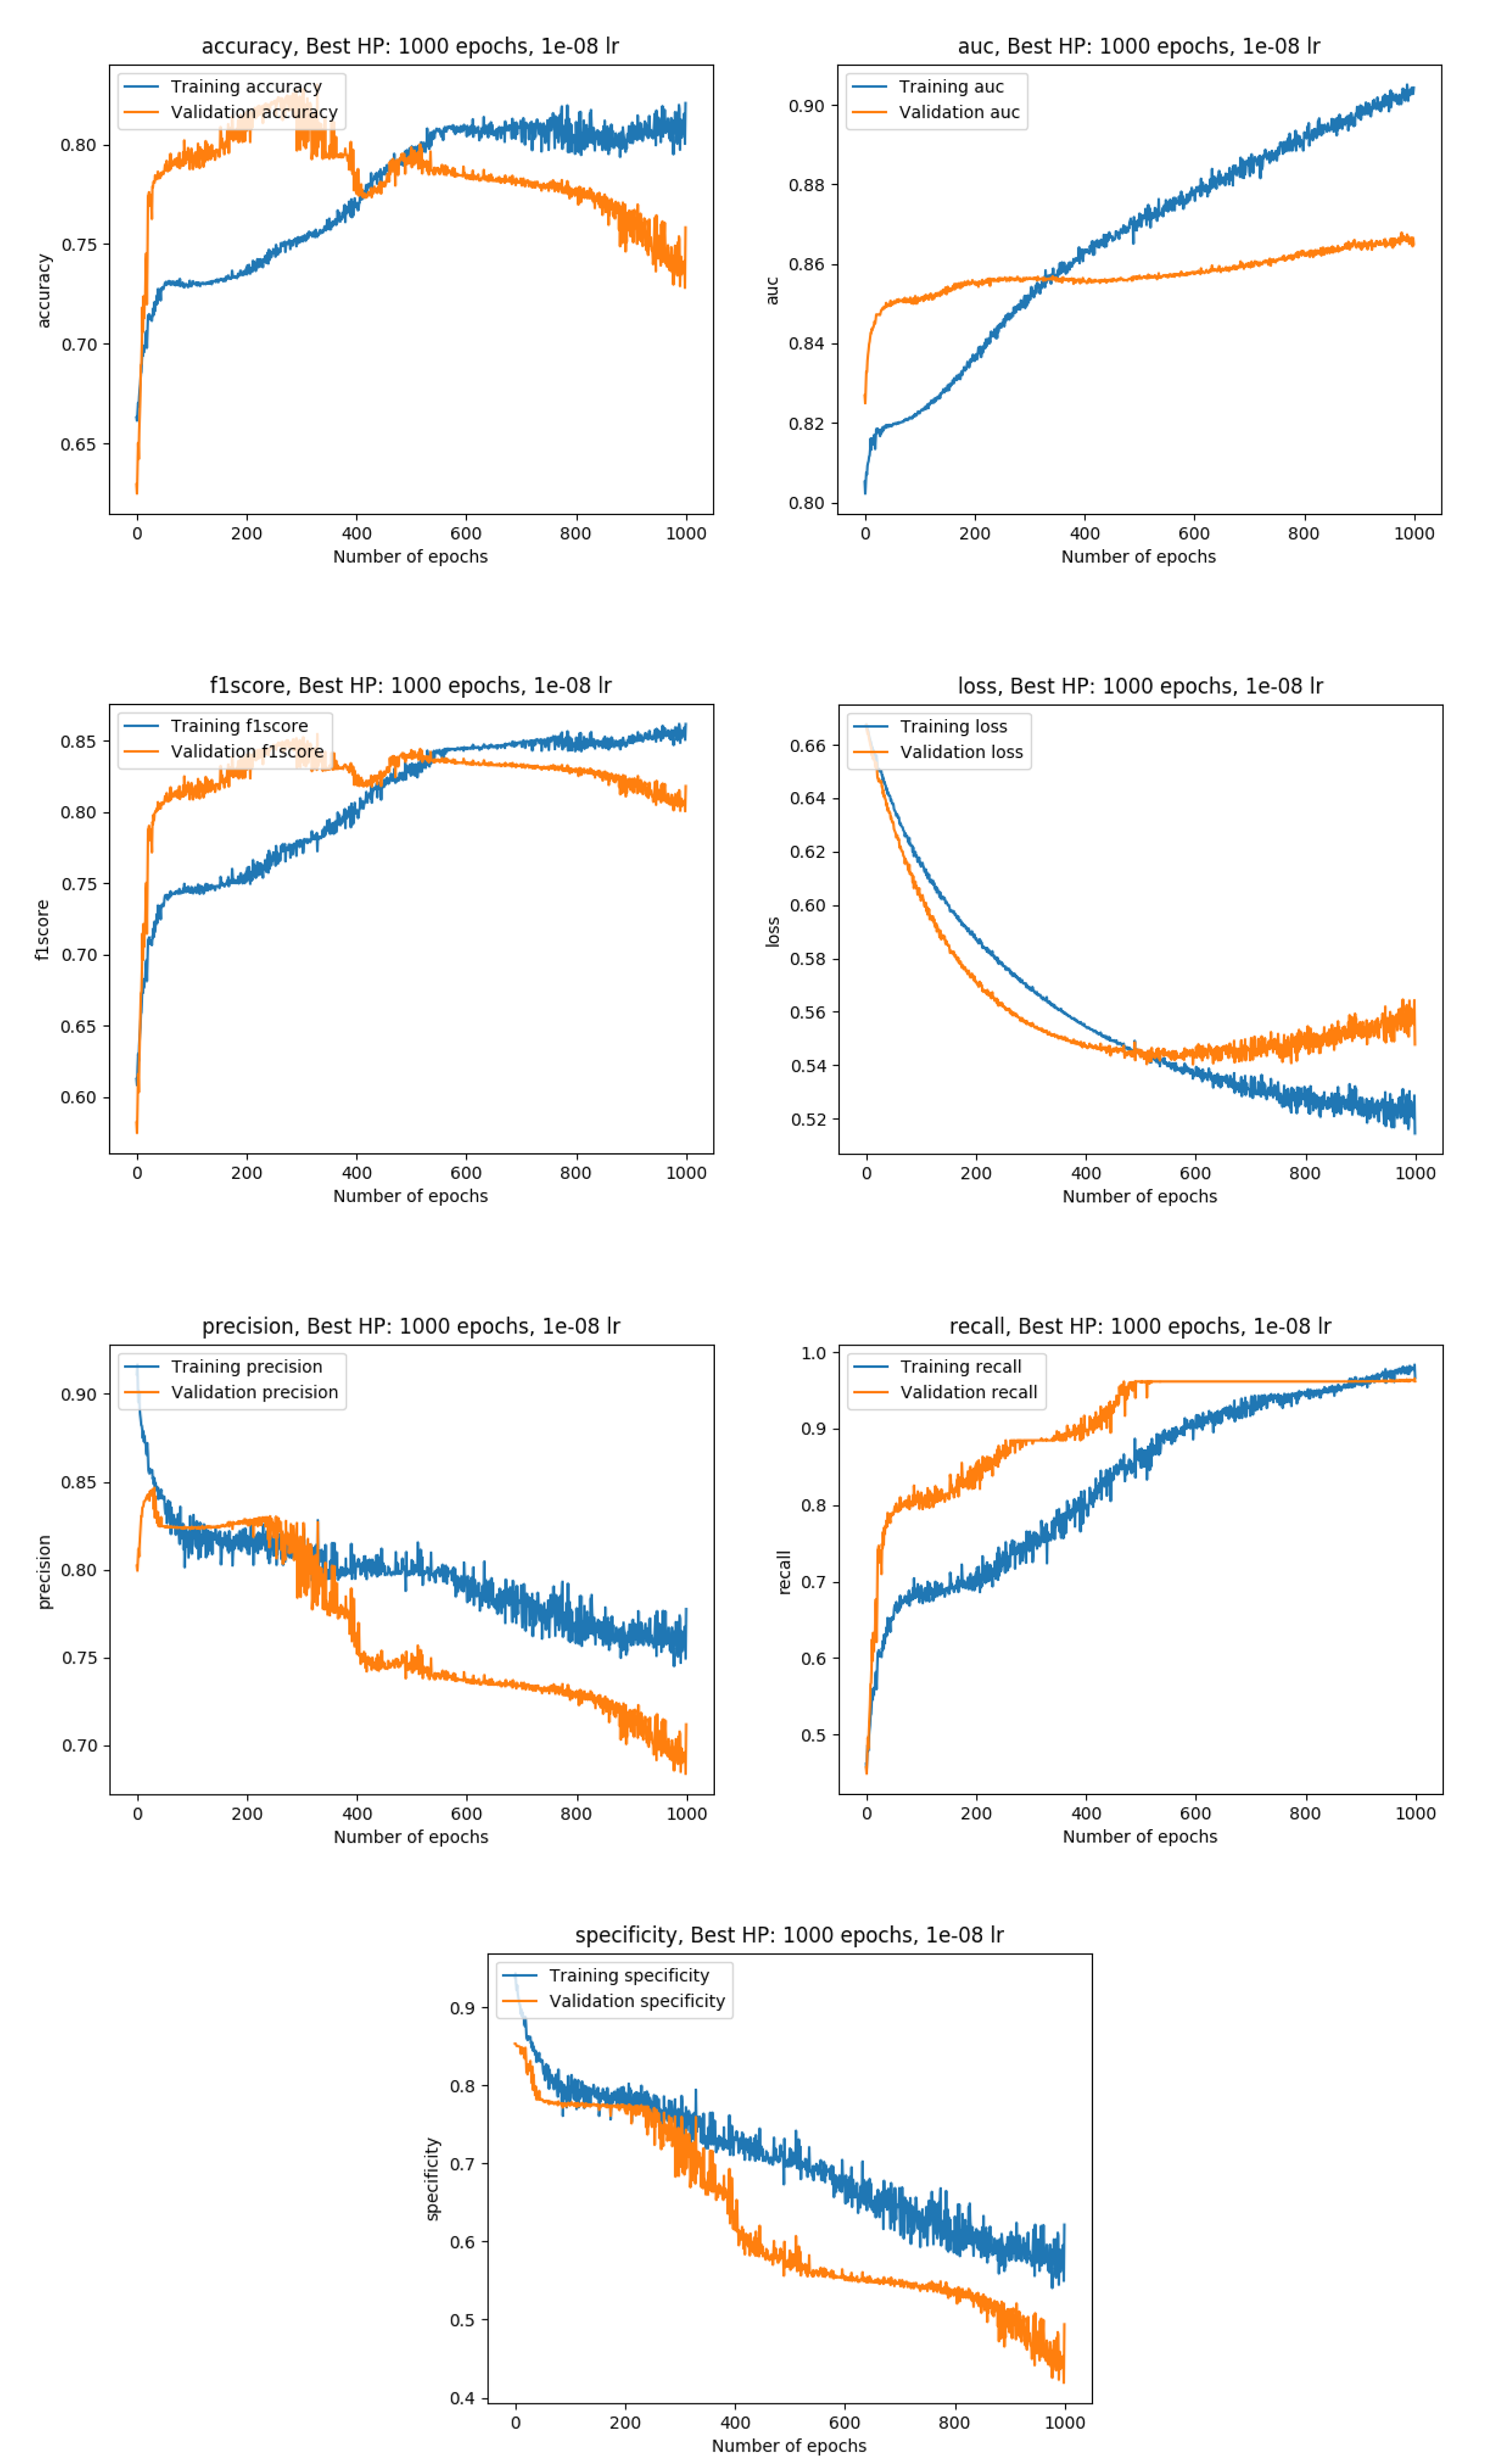
\includegraphics[width=0.95\textwidth, keepaspectratio=true]{./figures/tl_DS2_full.png}
}
\caption{Transfer learning - DS2 Full}
\label{fig:tl_ds2_full}
\end{figure}

\begin{figure}[!t]
\centering
\noindent
\makebox[\textwidth]{
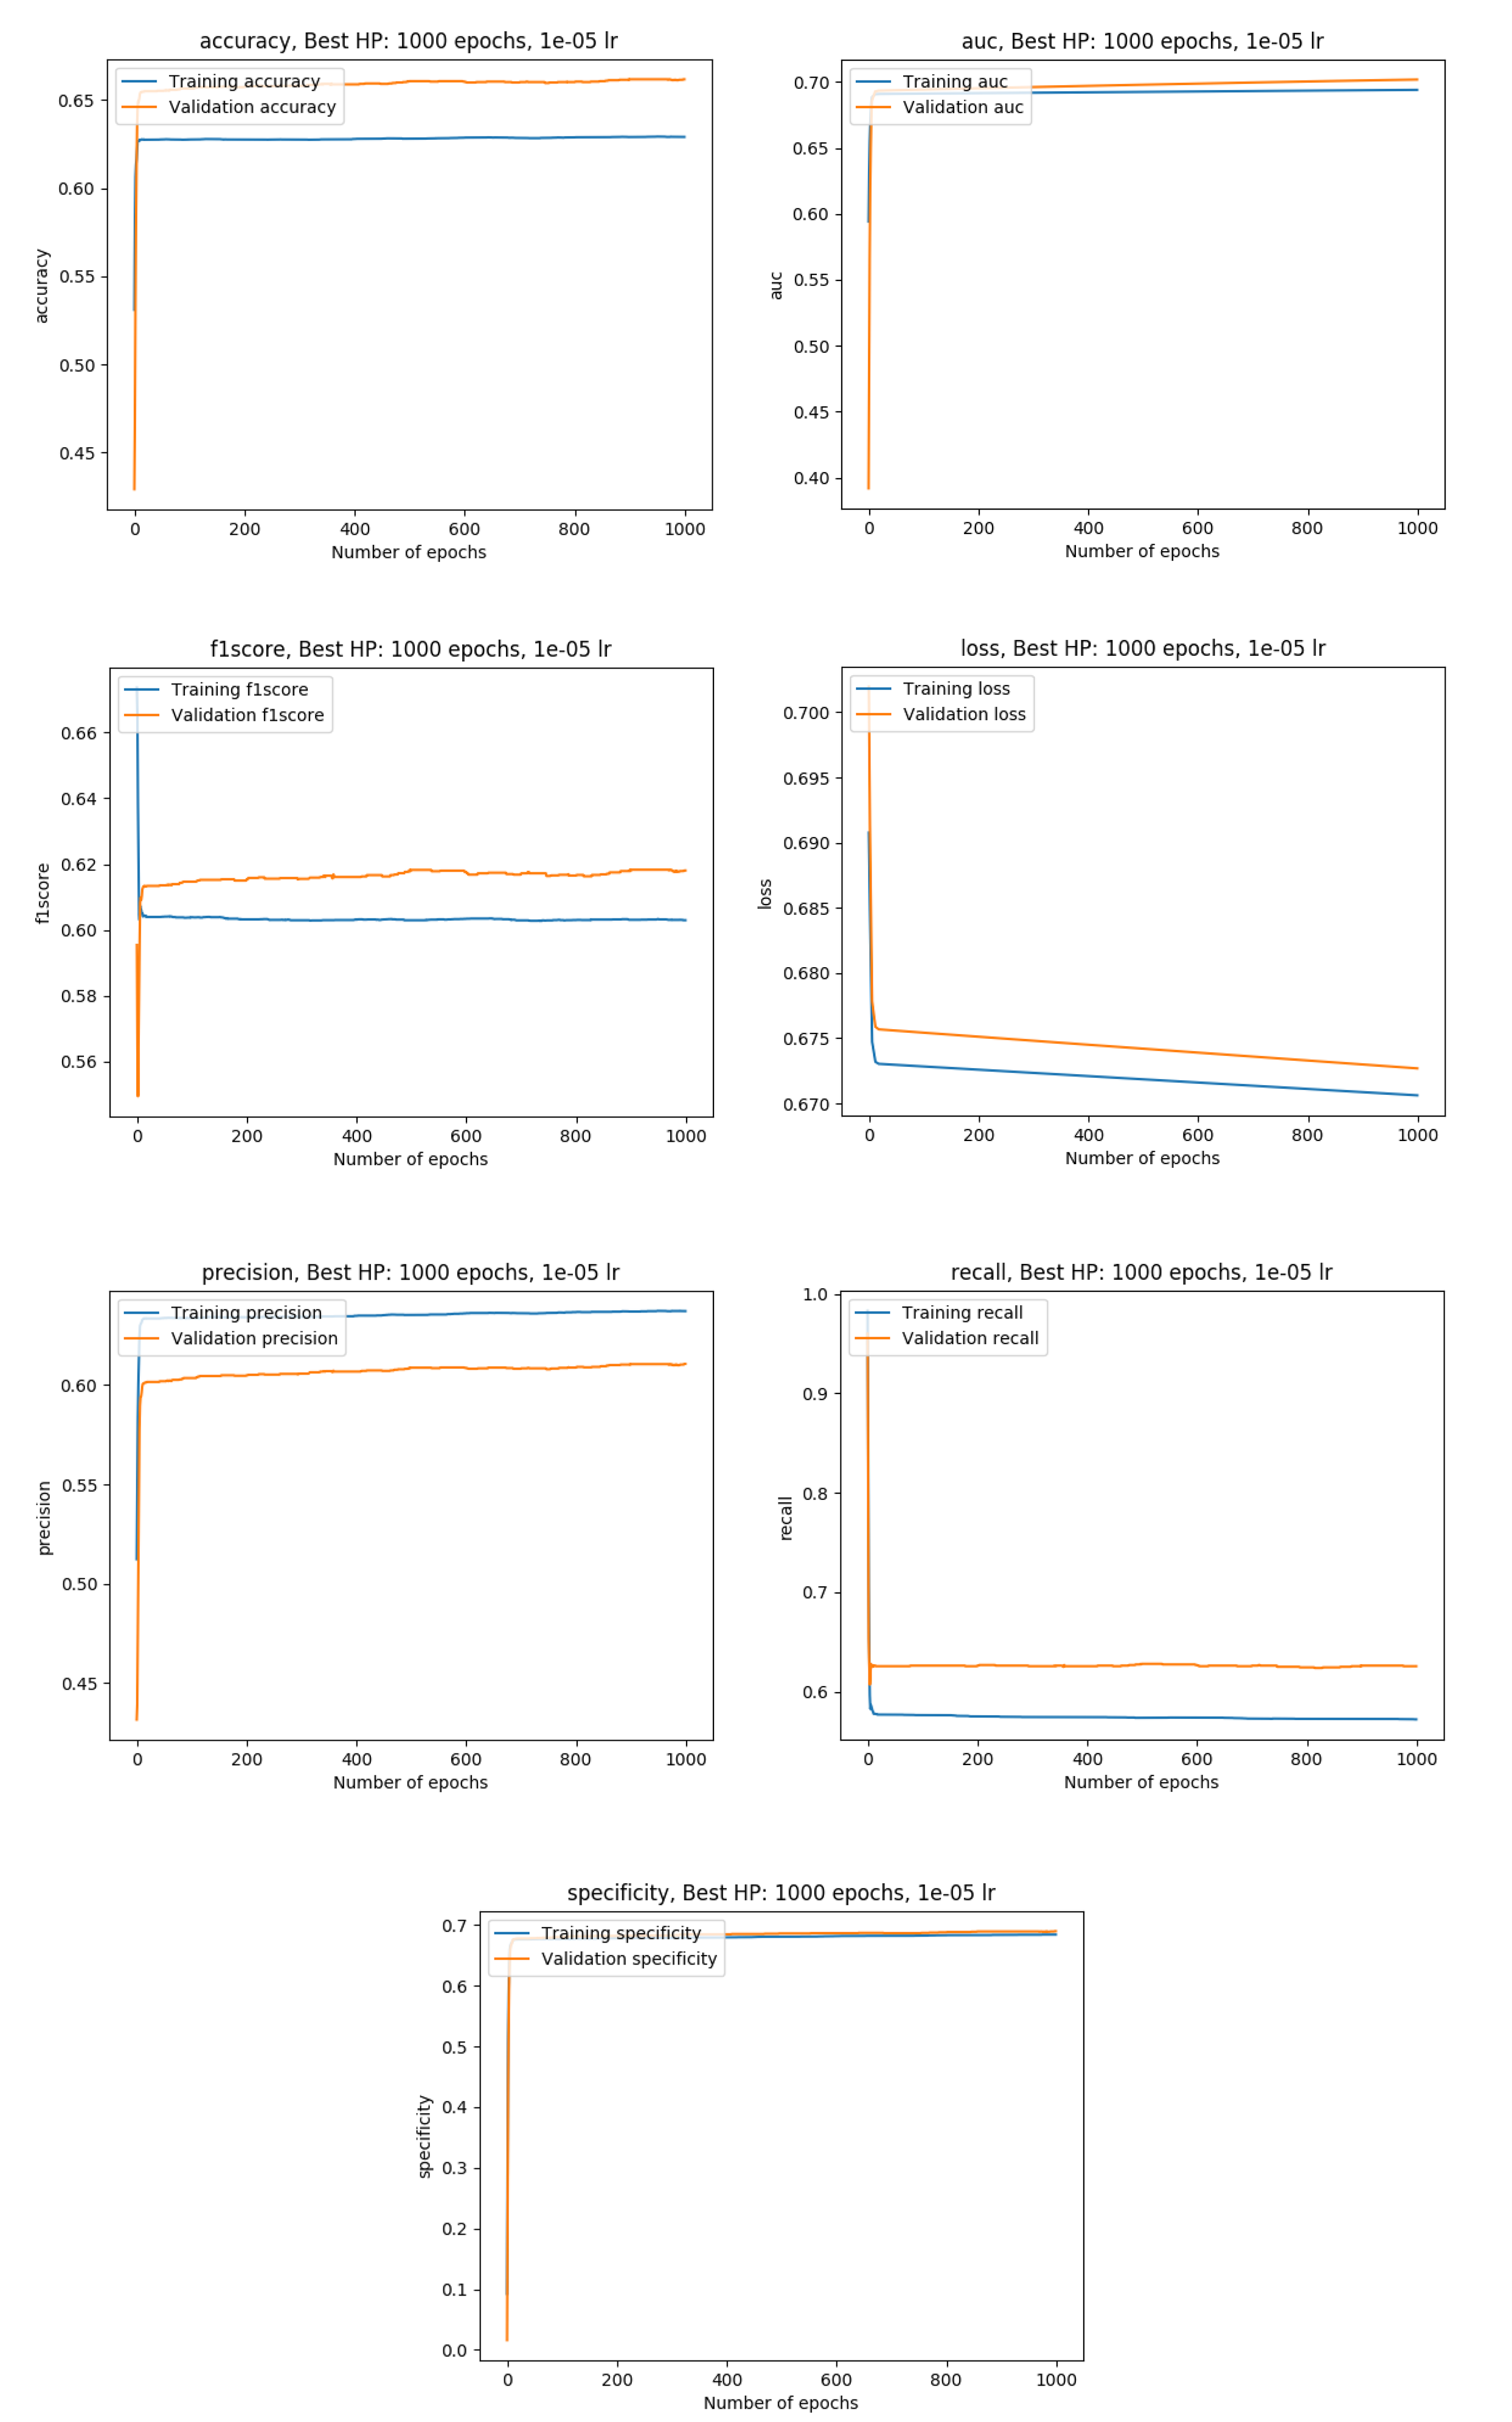
\includegraphics[width=0.98\textwidth, keepaspectratio=true]{./figures/tl_DS3_frozen.png}
}
\caption{Transfer learning - DS3 Frozen}
\label{fig:tl_ds3_frozen}
\end{figure}

\begin{figure}[!t]
\centering
\noindent
\makebox[\textwidth]{
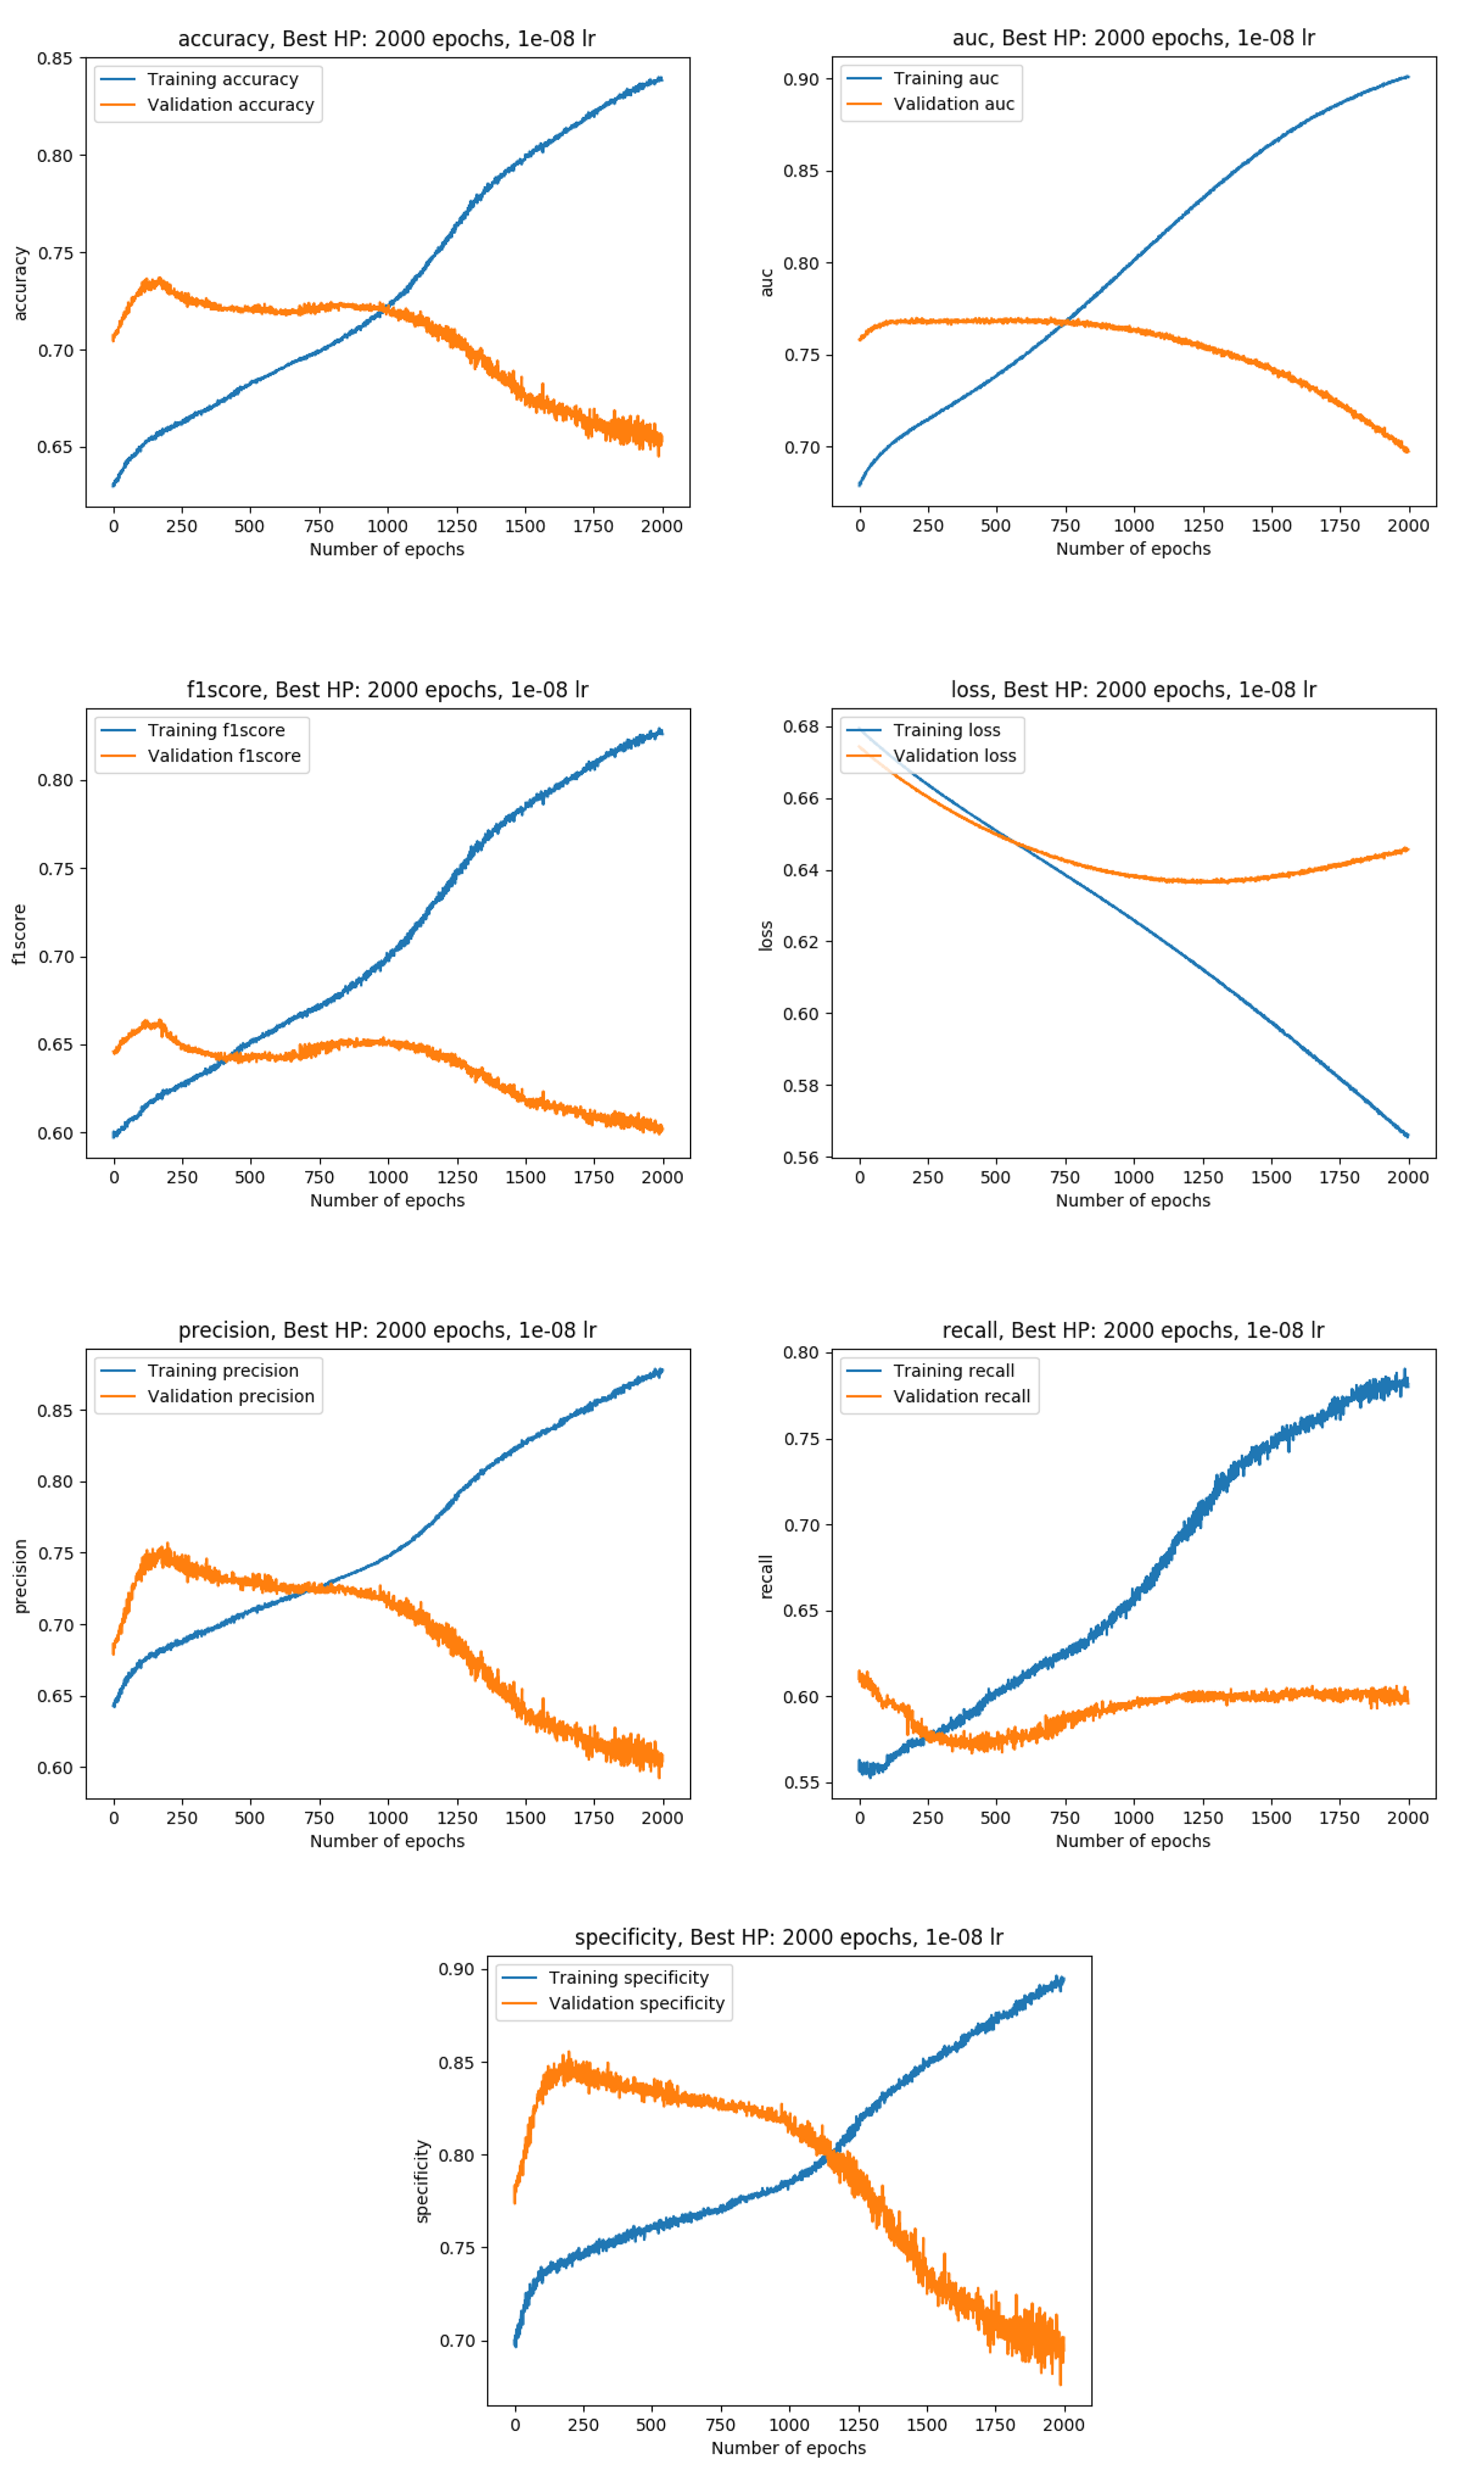
\includegraphics[width=0.98\textwidth, keepaspectratio=true]{./figures/tl_DS3_full.png}
}
\caption{Transfer learning - DS3 Full}
\label{fig:tl_ds3_full}
\end{figure}

\begin{figure}[!t]
\centering
\noindent
\makebox[\textwidth]{
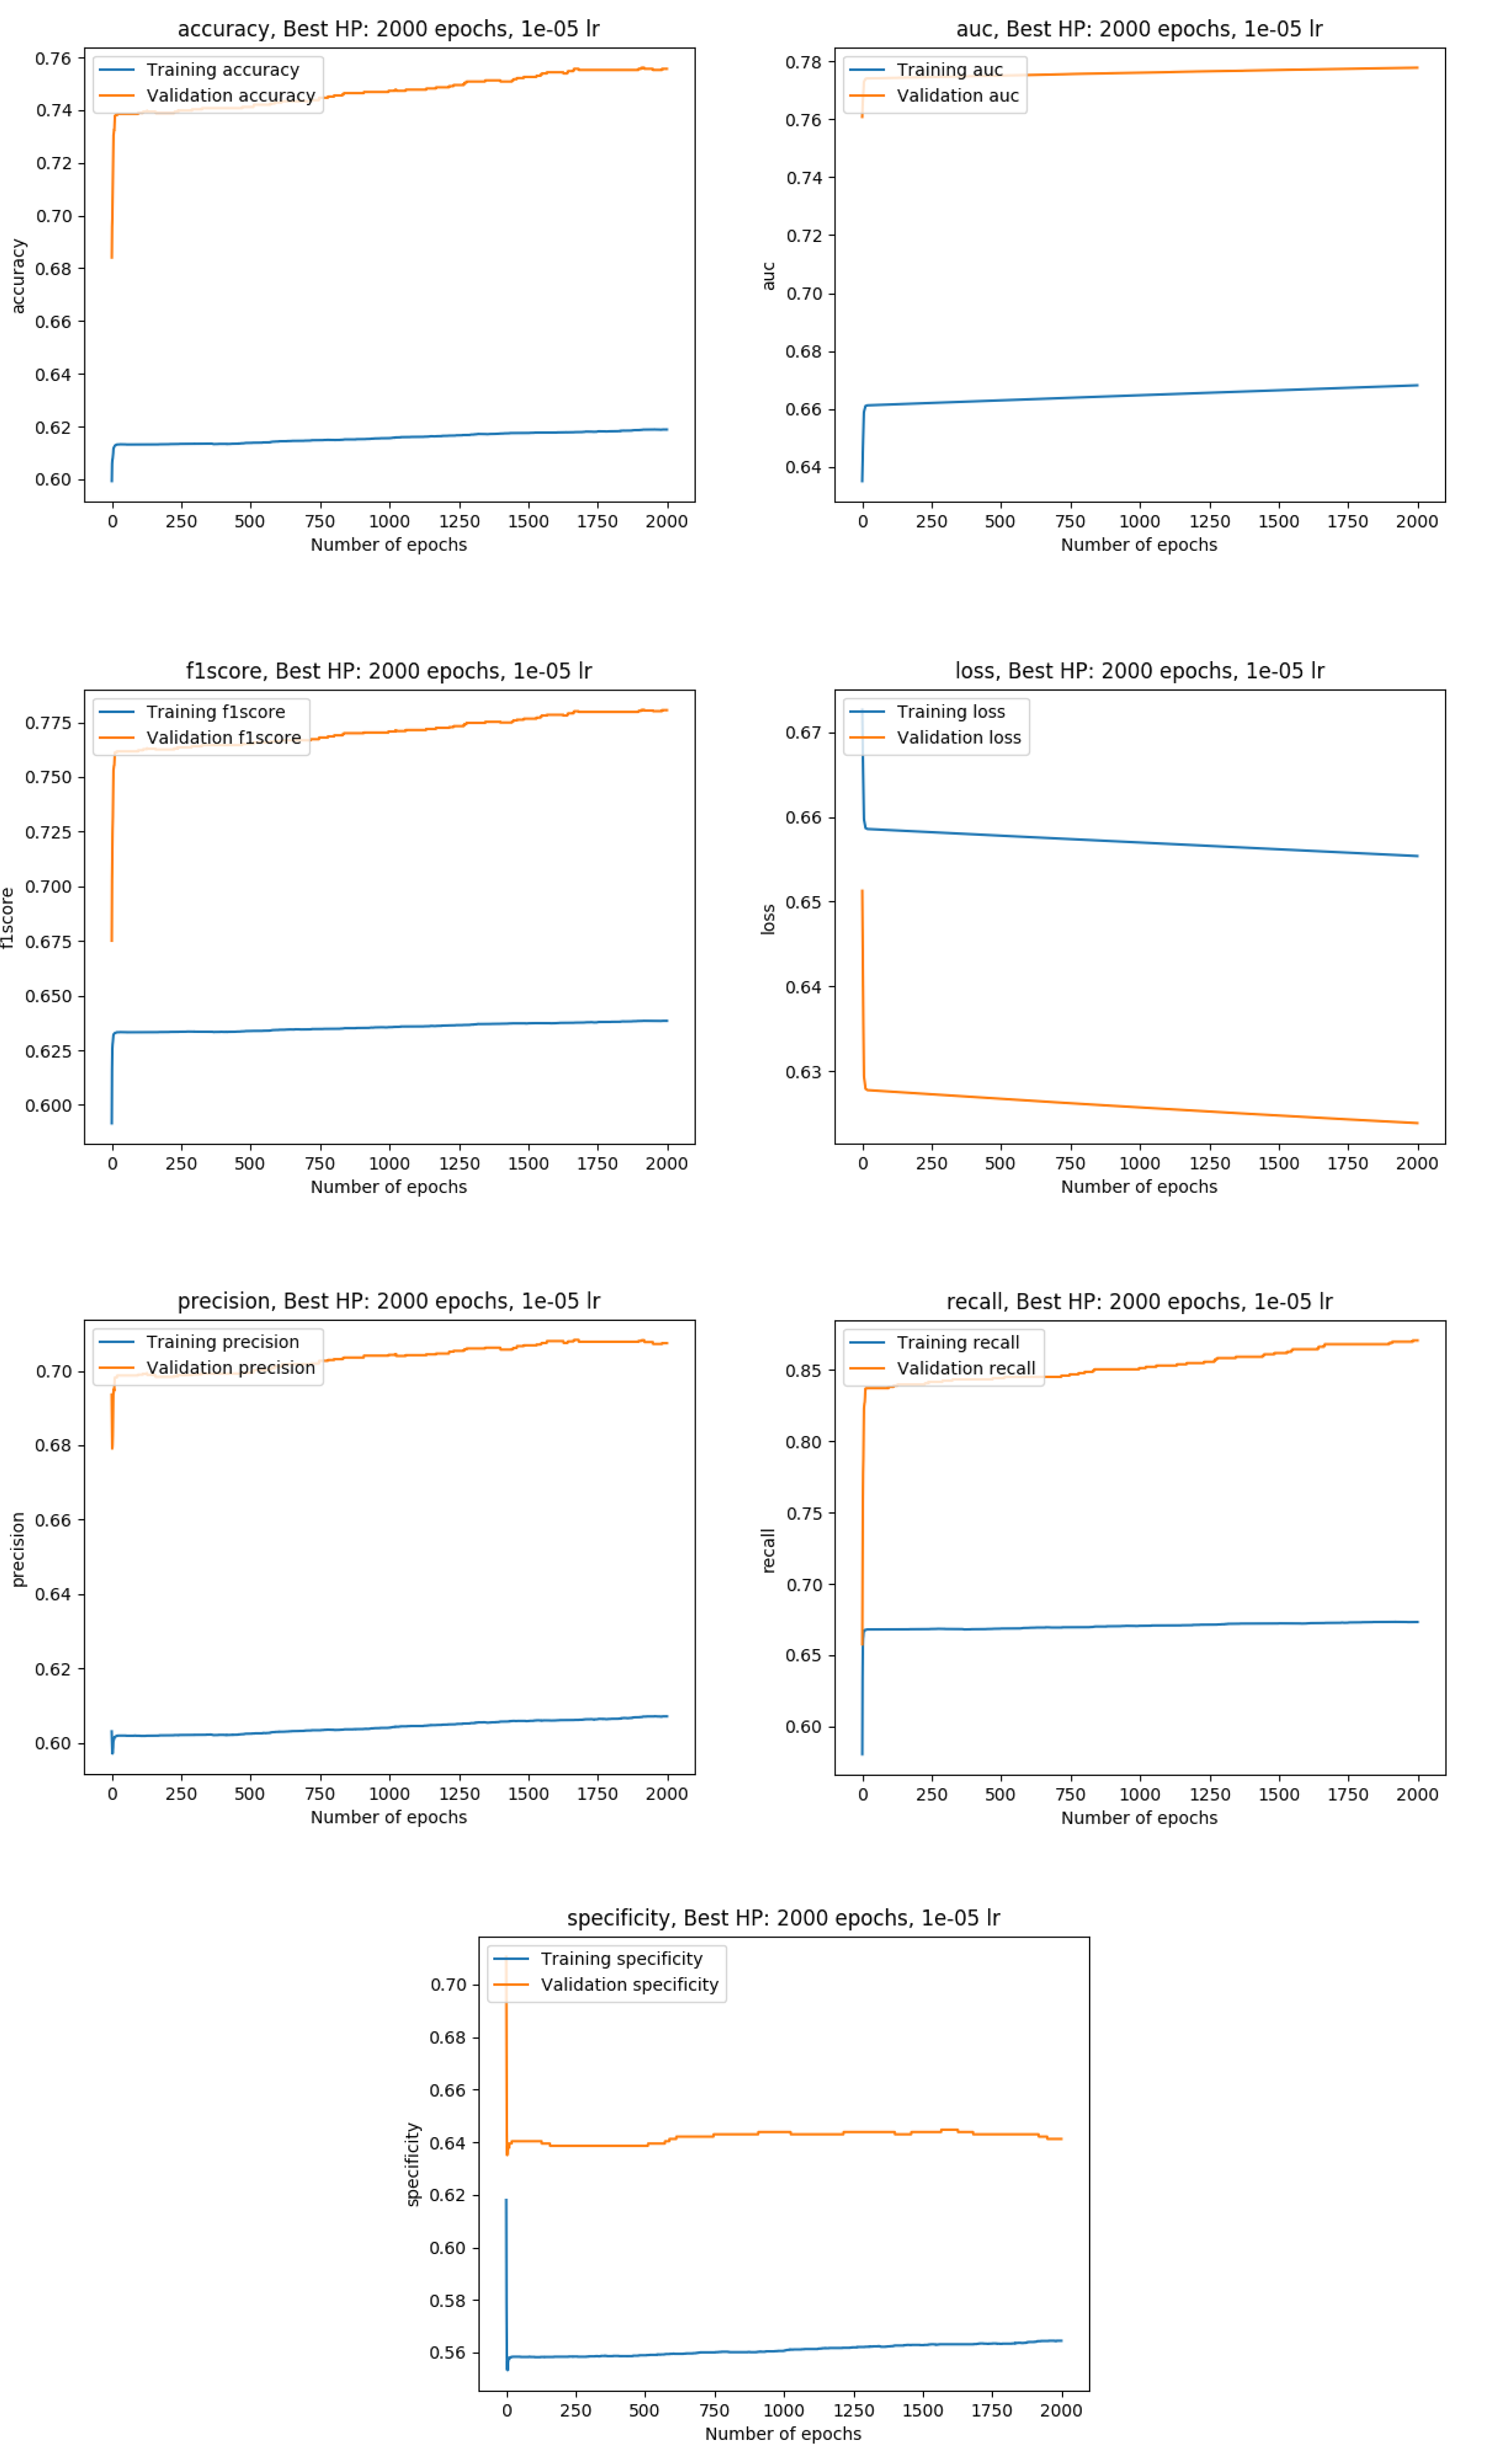
\includegraphics[width=0.98\textwidth, keepaspectratio=true]{./figures/tl_DS4_frozen.png}
}
\caption{Transfer learning - DS4 Frozen}
\label{fig:tl_ds4_frozen}
\end{figure}

\begin{figure}[!t]
\centering
\noindent
\makebox[\textwidth]{
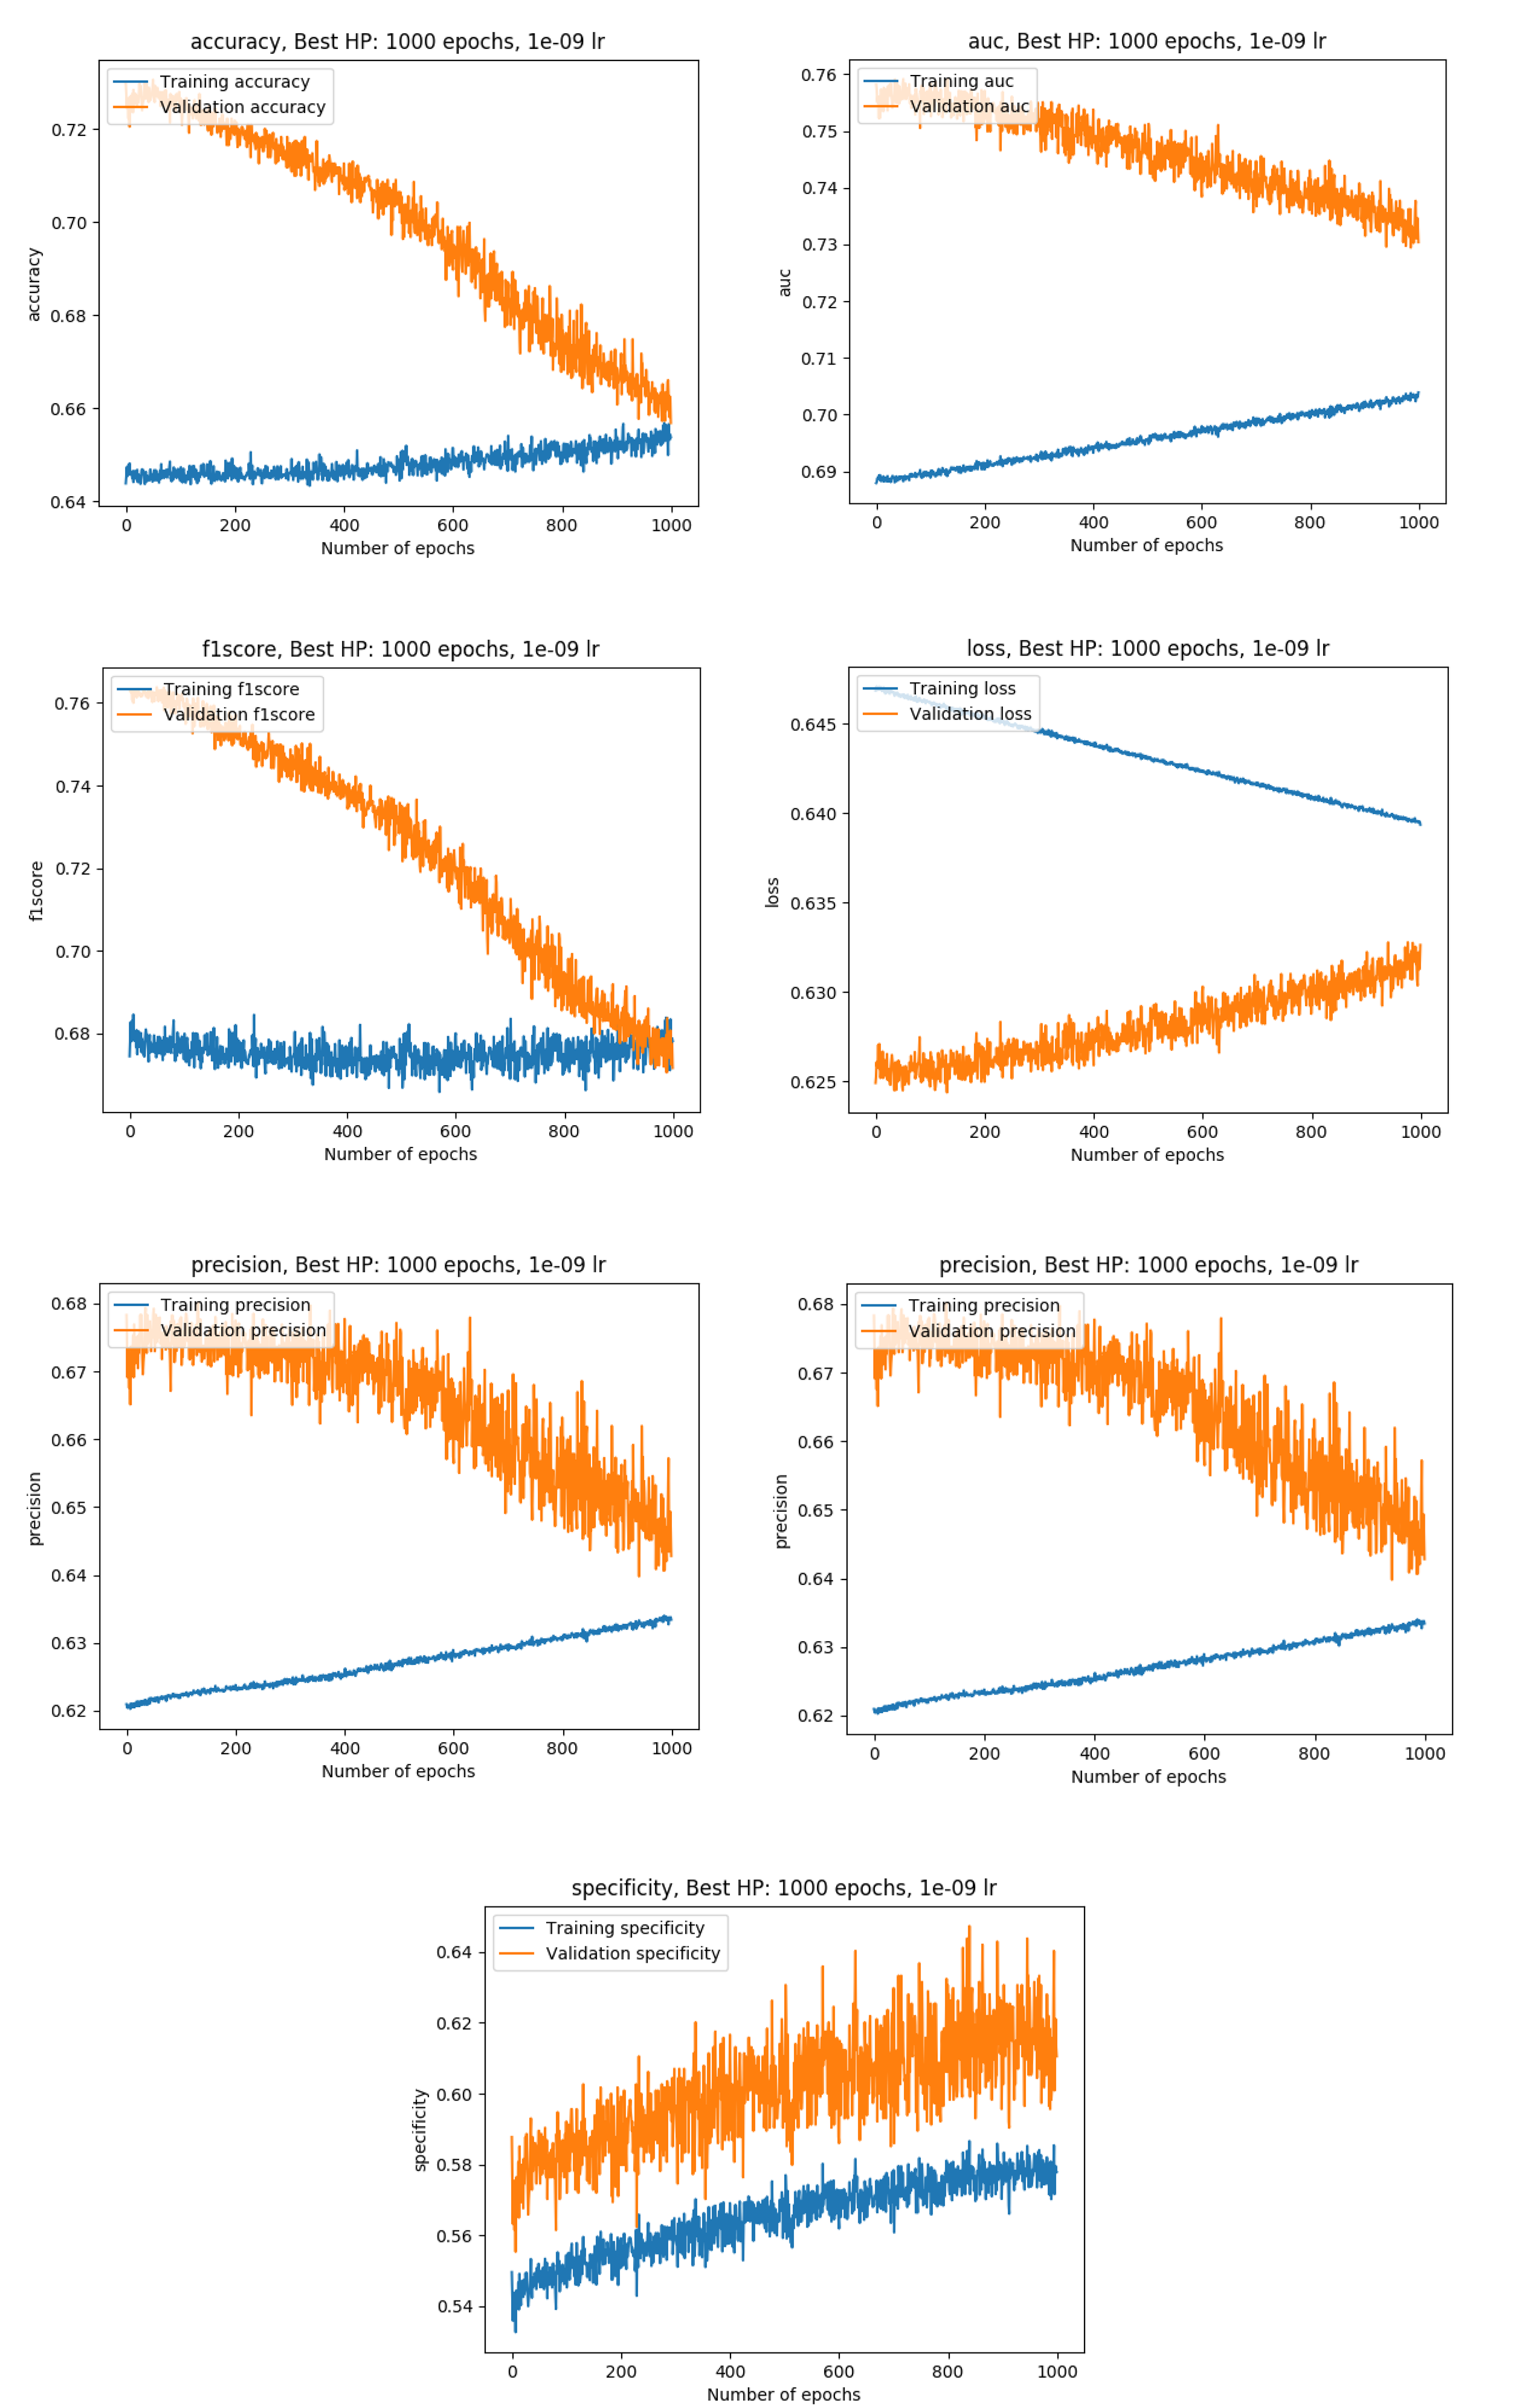
\includegraphics[width=1\textwidth, keepaspectratio=true]{./figures/tl_DS4_full.png}
}
\caption{Transfer learning - DS4 Full}
\label{fig:tl_ds4_full}
\end{figure}


\begin{table}[!t]
\resizebox{\textwidth}{!}{%
\begin{tabular}{|l|l|c|l|c|}
\hline
\rowcolor[HTML]{DAE8FC} 
\multicolumn{1}{|c|}{\cellcolor[HTML]{DAE8FC}\textbf{Dataset name}} & \multicolumn{1}{c|}{\cellcolor[HTML]{DAE8FC}\textbf{Step}} & \textbf{Best model saved at nth epoch} & \multicolumn{1}{c|}{\cellcolor[HTML]{DAE8FC}\textbf{Best model on the validation set}} & \textbf{Best model on the set set}                                                                                                                                      \\ \hline
\textbf{PROSTATEx}                                                  & DS1/Full                                                   & 527                                    & \begin{tabular}[c]{@{}l@{}}Accuracy: 0.6375\\ AUC: 0.7334\end{tabular}                 & \multicolumn{1}{l|}{\begin{tabular}[c]{@{}l@{}}Accuracy: 0.6842\\ Precision: 0.3333\\ Recall: 0.5000\\ F1-score: 0.4000\\ Specificity: 0.7333\\ AUC: 0.6833\end{tabular}}     \\ \hline
\textbf{Kaggle Brain}                                               & DS2/Frozen                                                 & 1999                                    & \begin{tabular}[c]{@{}l@{}}Accuracy: 0.7498\\ AUC: 0.8483\end{tabular}                 & -                                                                                                                                                                       \\ \hline
\textbf{Kaggle Brain}                                               & DS2/Full                                                   & 166                                    & \begin{tabular}[c]{@{}l@{}}Accuracy: 0.8172\\ AUC: 0.8596\end{tabular}                 & -                                                                                                                                                                       \\ \hline
\textbf{LungCTChallenge}                                            & DS3/Frozen                                                 & 1852                                    & \begin{tabular}[c]{@{}l@{}}Accuracy: 0.6734\\ AUC: 0.7755\end{tabular}                 & -                                                                                                                                                                       \\ \hline
\textbf{LungCTChallenge}                                            & DS3/Full                                                   & 167                                    & \begin{tabular}[c]{@{}l@{}}Accuracy: 0.7367\\ AUC: 0.7691\end{tabular}                 & -                                                                                                                                                                       \\ \hline
\textbf{PROSTATEx}                                                  & DS4/Frozen                                                 & 1914                                    & \begin{tabular}[c]{@{}l@{}}Accuracy: 0.7561\\ AUC: 0.7777\end{tabular}                 & -                                                                                                                                                                       \\ \hline
\textbf{PROSTATEx}                                                  & DS4/Full                                                   & 391                                     & \begin{tabular}[c]{@{}l@{}}Accuracy: 0.7662\\ AUC: 0.7749\end{tabular}                 & \multicolumn{1}{l|}{\begin{tabular}[c]{@{}l@{}}Accuracy: 0.6842\\ Precision: 0.3333\\ Recall: 0.5000\\ F1-score: 0.4000\\ Specificity: 0.7333\\ AUC: 0.8000\end{tabular}} \\ \hline
\end{tabular}%
}
\caption{Best model performance at each step of the transfer learning pipeline}
\label{table:tl_best_model_performance}
\end{table}




\section{Discussion}

\subsection{Training}
\setlength{\marginparwidth}{3cm}\leavevmode \marginnote{\textbf{Cl{\'e}ment}}This transfer learning experiment was performed manually. This means that each step was run sequentially, each time tuning the hyperparameters (learning rate and dropout probability) to reach the best performance possible.

First of all, the best weight initialization among 200 random initializations was loaded and trained on the PROSTATEx dataset. With a learning rate of $1*10^{-8}$ and a dropout of $0.4$, the model learned genuine features in a smooth way (accuracy of $0.6340$ and AUC of $0.7359$ on the validation set). Obviously, the values are lower than the ones reached in Section \ref{sec:paper_reproduction_results} (accuracy of $0.7525$ and AUC of $0.765$) since the current experiment only uses DWI images. Hence, this model could only learn from one third of the information the first model had at disposal. Furthermore, the training and validation curves remained close during the whole experiment. This behavior indicates that the model actually learns features on the training set and generalizes well on new data (validation set), which is the best case scenario.

Second, the first frozen training took place on the brain dataset. During the first epochs, the metrics remained low. For example, the accuracy was below $0.5$, which means that a model classifying the input randomly would have performed better. This was expected since the last layers were reset to new random initialization. In these early stages, the model was relying on a feature extractor capable of classifying prostate cancer and a new decision maker which did not have the time to adapt to the new task. Thanks to a learning rate of $1*10^{-7}$ and a dropout probability of $0.3$, the metrics started increasing early, reaching impressive values (accuracy of $0.7799$ and AUC of $0.8379$). Since the feature extractor is frozen, this behavior indicates that the features allowing to detect prostate cancer transfer well to brain cancer. Once more, the training and validation curves have the same shape for every metric, which implies a healthy learning process.

% Mention no reducelr ?
Then, the full model was trained on the same dataset. The model resulting from the previous set was composed of decision maker trained on this dataset and a feature extractor resulting from the training on the prostate dataset (whose features seem to suit this dataset well). Therefore, the first metric values are already high. The rest of the training aimed at learning new useful features from the brain images, which could then be used for lung and prostate cancer classification. As expected, this step increased the metrics a bit (accuracy of $0.8233$ and AUC of $0.8566$).

The model was then frozen again and trained on the third dataset composed of lung images. Here again, the metrics peaked early. This is partly due to the larger learning rate of $1*10^{-5}$ and to the common features that prostate, brain and lung cancers share. The metrics went not as high as for the brain dataset but still showed good signs of the usefulness of the prostate and brain features.

The full training on the lung dataset went smoothly and allowed to increase the accuracy by $0.03$ and the AUC by $0.2$ before reaching stability.

Finally, the model was trained on the first dataset again. At the beginning of the frozen part, the last layers were not initialized randomly. In fact, the last layers coming from the model resulting from the training on the first dataset were used as last layers. Since these last layers were already trained on the same dataset, the improvement occuring during this training stemed from new features learned from the brain and lung datasets. Even with a large learning rate of $1*10^{-5}$, the curves went up slowly and regularly throughout the whole training. Therefore, the features acquired thanks to transfer learning are really helpful for the prostate cancer classification.

Regarding the full training, the curves contain quite some noise with a already small learning rate of $1*10^{-9}$. An even smaller learning rate of $1*10^{-10}$ was tested and it turned out to be too small since the training and validation curves were completely flat from the beginning to the end. Here, the validation curves show an improvement during the first 50 epochs approximately, before going down while the training metrics keeps increasing. At this point, the model reached its optimum. Moreover, the fact that the validation metrics are much higher than the training ones with a dropout probability of 0.0 indicates that the model generalizes well thanks to transfer learning. 


\subsection{Visualization of the impact of the various datasets on the target task}
\setlength{\marginparwidth}{3cm}\leavevmode \marginnote{\textbf{Cl{\'e}ment}}Figure \ref{fig:tl_global_validation_auc} shows the evolution of the AUC on the validation set of PROSTATEx. As expected, the first training on PROSTATEx generated the same curve as on Figure \ref{fig:tl_ds1_full}. The latter looks steeper because of the difference in the X-axis scale.

Moreover, the frozen training on the second dataset (as well as the other frozen trainings) shows a flat line. Reason for that is that the feature extractor and the decision maker do not change here. In fact, the former is frozen and the latter is always the same. As the decision maker is the one coming from the best model of the first training according to the validation AUC, the flat line is as high as the best validation AUC value reached during the first training.

Furthermore, the full training curve shows that brain cancer features are actually helpful. If they were not, the metric would not have increased as fast and would not have reached such values.

During the full training on the lung dataset, the AUC starts at a high value after the first epoch. The combination of the prostate, brain and lung features seem to help the model generalize. This hypothesis is confirmed by the values reached during last training on the prostate dataset. In fact, the AUC value is higher than the one reached during the first training. Interestingly, the curve starts high, improves for 50 epochs and starts decreasing. This implies that the model reached a high level of generalization during transfer learning. These 50 epochs were enough to keep the low level features learned thanks to the other datasets while adapting the model to the target task again. 

%\subsection{Visualization of the impact of the various datasets on the target task}
%\label{sec:global_performance}
%\setlength{\marginparwidth}{3cm}\leavevmode \marginnote{\textbf{Julien}}On paper, each step of the transfer learning is supposed to make the model learn new features that are useful for the first dataset (the target dataset). As described in section \ref{sec:process_overview}, the model can be seen as a feature extractor and a decision maker. Hence, to see how much each step was actually helping the process, the decision maker resulting from the first step of the transfer learning, i.e. the training on the first/target dataset, was saved. As this decision maker is saved after the training on the target dataset, it is specialized in the classification of the latter. In other words, if the target dataset is a prostate dataset, it will classify prostate tumors with a relatively high precision. 
%
%Then, after each epoch of every other transfer learning step, the saved decision maker was attached to the current feature extractor. This temporary model was then tested on the target training and validation sets, which resulted in different training and validation metrics. 
%
%At the end of the transfer learning pipeline, a graph was generated for each metric. These curves show the evolution of the latter across the entire process, which allows to determine the impact of each non-target dataset on the target task. If a metric is increasing, the features learned thanks to the corresponding dataset are useful for the target one. Figure \ref{fig:global_performance_example} shows an example of this graph for the AUC.\\
%As expected, the curve is flat during the frozen parts. Since the same decision maker is attached to frozen layers (which remain the same by definition), the values of the metrics do not change at all.


%To draw these graphs, a temporary model was created and tested at the end of each epoch. The latter is composed of the current feature extractor attached to the decision maker of the best model resulting from the first training on the prostate dataset. Doing so ensures that the model is able to classify prostate cancer (thanks to the trained decision maker) but making use of the features learned during transfer learning exclusively.\\
%The frozen steps are flat lines since the feature extractor and the decision maker do not change here. In fact, the former is frozen and the latter is always the same. 

\begin{figure}[!h]
\centering
\noindent
\makebox[\textwidth]{
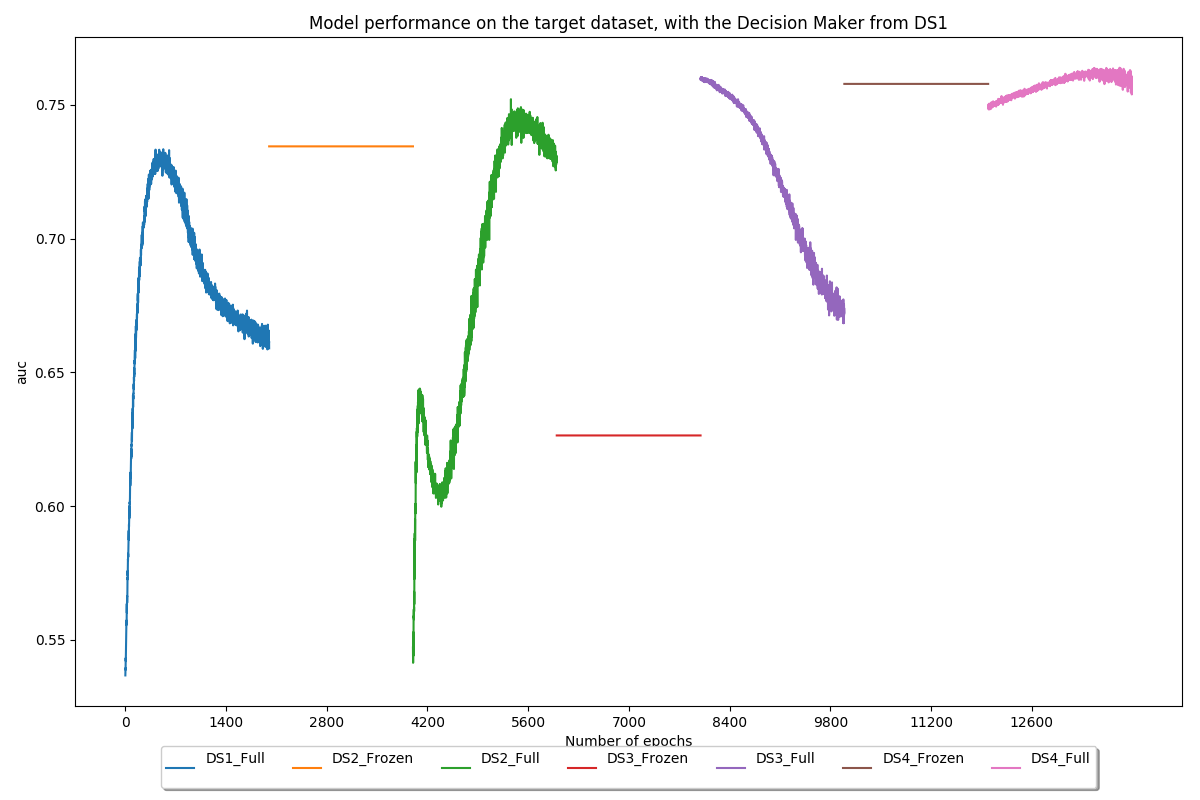
\includegraphics[width=1\textwidth, keepaspectratio=true]{./figures/tl_global_validation_auc.png}
}
\caption{Transfer learning - Global Performance - Validation AUC}
\label{fig:tl_global_validation_auc}
\end{figure}


\subsection{Testing}
\setlength{\marginparwidth}{3cm}\leavevmode \marginnote{\textbf{Cl{\'e}ment}}To test the effectiveness of this transfer learning pipeline, the performance of the model before and after transfer learning was compared. Figure \ref{fig:tl_results_test_set} summarizes the various metrics. To obtain these numbers, both models were tested on our test set which has never been seen by the model before. The transfer learning allowed to increase every single metric. First, the AUC increased by approximately 10\%, going from $0.68$ to $0.77$. The recall went from $0.5$ to $0.75$. Both metrics are key metrics in a medical context. In fact, classifying a positive case as negative is far worse than the opposite. Hence, maximizing the AUC (which is an indicator of how well the model is able to differentiate each class) and the recall (which shows how many positive cases have been correctly detected by the model). Apart from these metrics, the accuracy gained around 10\% ($0.68$ to $0.74$). 


\begin{figure}[!h]
\centering
\noindent
\makebox[\textwidth]{
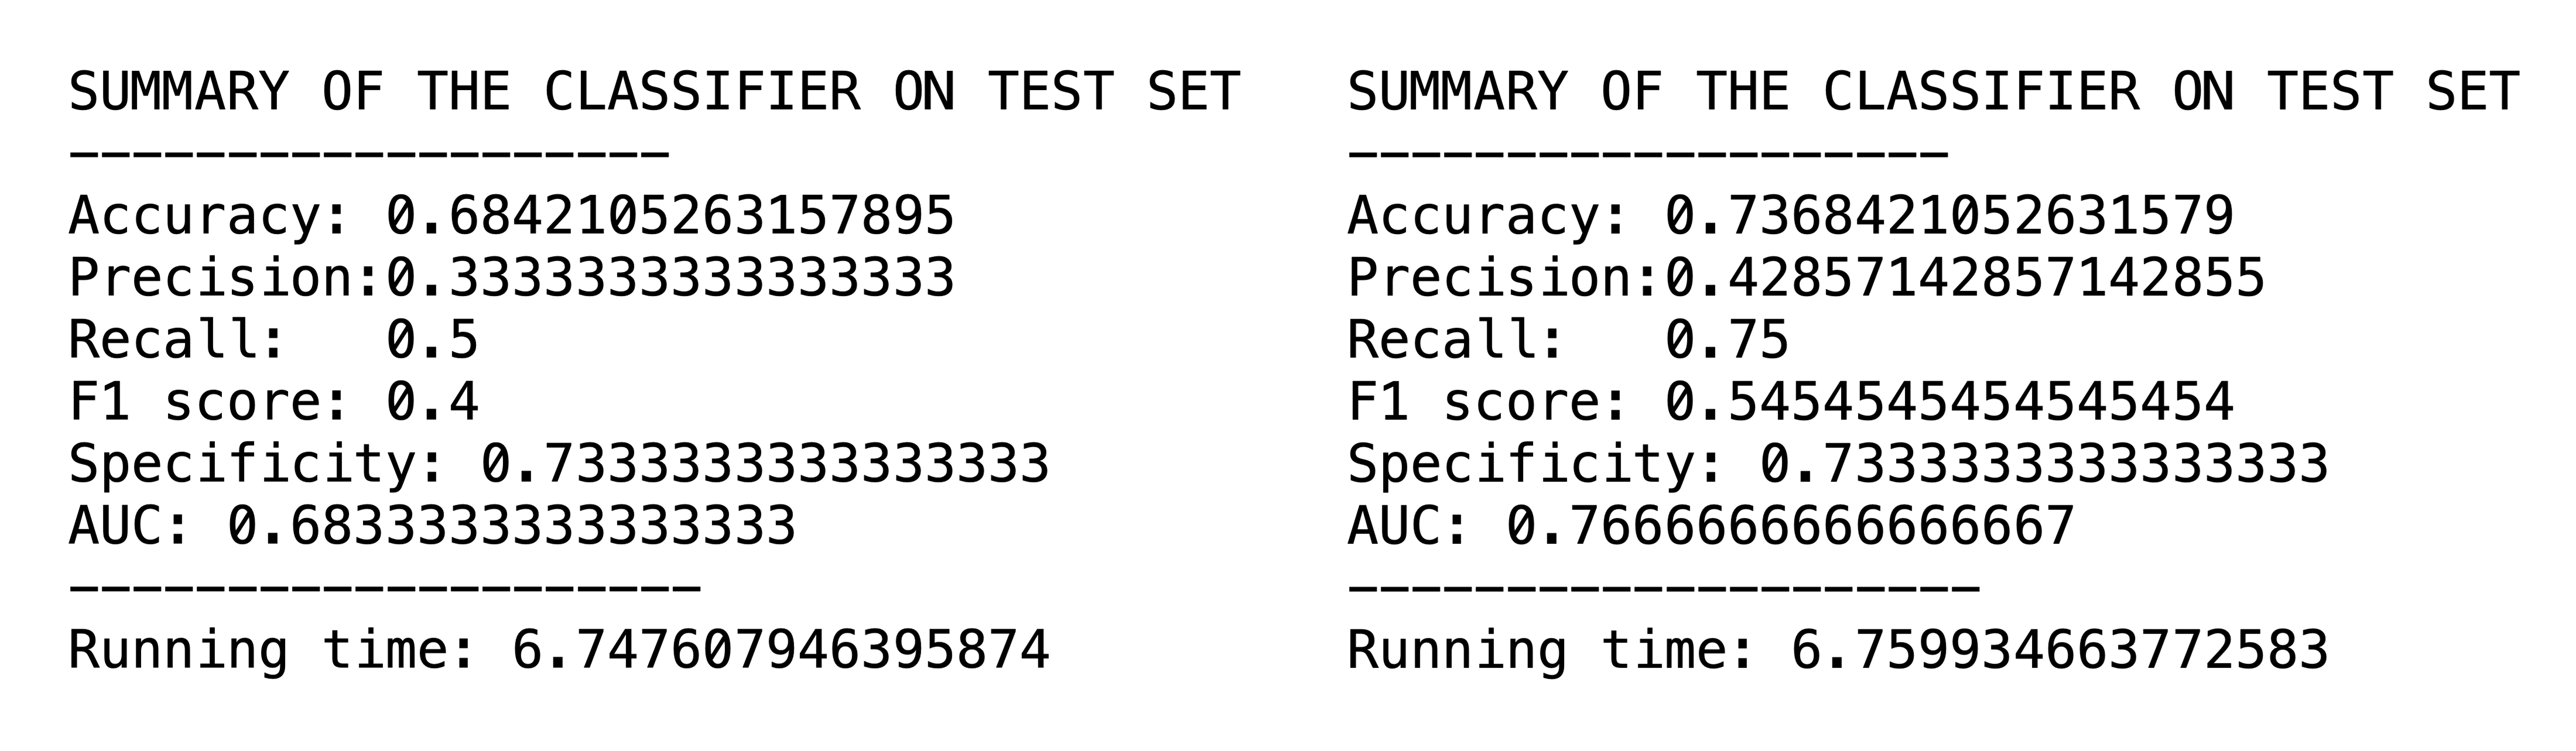
\includegraphics[width=1\textwidth, keepaspectratio=true]{./figures/tl_results_test_set.png}
}
\caption{Transfer learning - Performance comparison between the best model obtained during DS1 Full and DS4 Full}
\label{fig:tl_results_test_set}
\end{figure}


\subsection{Conclusion}
\setlength{\marginparwidth}{3cm}\leavevmode \marginnote{\textbf{Cl{\'e}ment}}This transfer learning approach using frozen and unfrozen parts allowed to increase the performance of the model up to 10\% depending on the metric. Moreover, it also increased the generalization ability of the model by learning features coming from different body parts. This makes the model more robust and more likely to classify new unseen data well. These improvements are a huge step forward in a field where the nonavailability of data is a real obstacle that prevents deep learning-based cancer classification systems from making a major breakthrough.

